\chapter{Literature Review}\label{chap:systematic_literature_review}

% Intro to the chapter
This Chapter presents the background required to better understand
this work and its literature review. Topics on Proteins are presented on
Section~\ref{sec:proteins}. Section~\ref{sec:psp} contains the literature
review on the Protein Structure Prediction Problem. Section~\ref{sec:bioinspired}
presents the literature review for Optimization and Bio-Inspired algorithms.
Section~\ref{sec:related_works} presents the related works.

\section{Proteins}~\label{sec:proteins}

% What are proteins
Proteins are macromolecules synthesized by the body with direct information from
the \ac{DNA}. The \ac{DNA} encodes an amino acid sequence, that when assembled correctly it
will originate the desired protein. Upon creation and shortly after the protein
assumes its native conformation. This conformation, i.e. the three dimensional
structure, is directly responsible for the protein function
\cite{lee2017ab}.

The process of protein assembly happens spontaneously, in a complex manner which
is not currently fully understood~\cite{dill2008protein}.
While each protein can be identified uniquely by
its amino acid sequence, it is possible that the protein folds incorrectly.
When this occurs the protein either can stop performing its
original functionality or assume a toxic state where it can harm cells,
tissues and even whole organs.
If this is a systematic issue then it is called a proteopathy.

\subsection{Amino Acids}~\label{sec:amino-acids}

% What are amino acids
The building blocks of proteins are amino acids. There are 20 known naturally
occurring amino acids with varying degrees of complexity. Of these, the human
body can only synthesize 10, and the other 10 must be externally supplied
(in the food). The lack of any of these amino acids will cause diminishing
body functions, as shown in~\cite{crews1969weight}.

% Amino acid structure
Amino acids are composed of a main Carbon atom, called the $\alpha$ Carbon
or $C_\alpha$, bound to 4 elements: An hydrogen atom; A Carboxyl Group; An
Amino Group; And a side chain, also named R-Group.
Figure~\ref{fig:amino-acid-structure} contains a visual representation of
an amino acid.

\begin{figure}
    \centering
    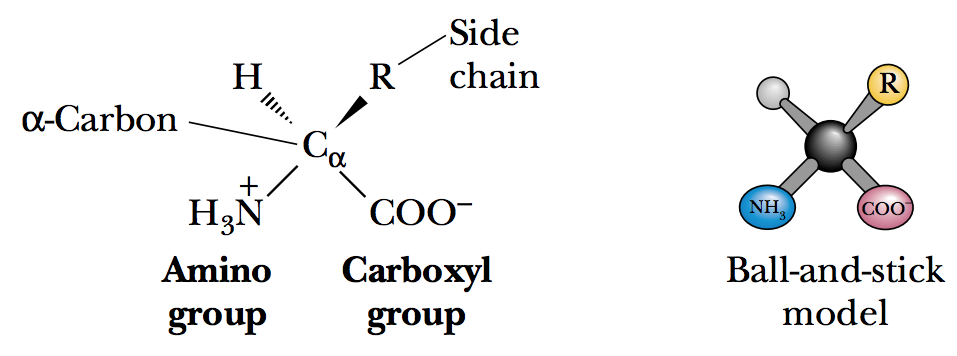
\includegraphics[width=0.7\textwidth]{Figuras/amino-acid.png}
    \caption{Amino Acid Structure (Source:~\cite{garrett1999biochemistry})}
    \label{fig:amino-acid-structure}
\end{figure}

Each amino acid has several designated identifications, as shown in
Table~\ref{tab:amino-acids}. The first column shows the amino acid name.
The second shows the 3 letter code. The third column shows the 1 letter code.
The 1 letter code is commonly used to describe amino acid sequences and
will be used throughout this work.

\begin{table}[h]
    \centering
    \begin{tabular}{c|c|c} \hline \hline
        Name          & 3 Letter Code & 1 Letter Code \\ \hline \hline
        Alanine       & Ala  & A \\
        Arginine      & Arg  & R \\
        Asparagine    & Asn  & N \\
        Aspartic acid & Asp  & D \\
        Cysteine      & Cys  & C \\
        Glutamic acid & Glu  & E \\
        Glutamine     & Gln  & Q \\
        Glycine       & Gly  & G \\
        Histidine     & His  & H \\
        Isoleucine    & Ile  & I \\
        Leucine       & Leu  & L \\
        Lysine        & Lys  & K \\
        Methionine    & Met  & M \\
        Phenylalanine & Phe  & F \\
        Proline       & Pro  & P \\
        Serine        & Ser  & S \\
        Threonine     & Thr  & T \\
        Tryptophan    & Trp  & W \\
        Tyrosine      & Tyr  & Y \\
        Valine        & Val  & V \\ \hline \hline
    \end{tabular}
    \caption{The 20 Naturally Occurring Amino Acids}
    \label{tab:amino-acids}
\end{table}

Each amino acid can be split into groups accordingly to its properties.
There are six commonly used groups~\cite{garrett1999biochemistry}:
The Aliphatic Hydrophobic; The Aromatic Hydrophobics; The neutrals;
The Basics (Positively Charged); The Acids (Negatively Charged);
and the Unique Amino Acids. The Aliphatic Hydrophobic group is composed of
Alanine, Isoleucine, Leucine, Methionine and Valine. The Aromatic Hydrophobic
is composed of Phenylalanine, Tryptophan and Tyrosine. The neutral group is made
out of Asparagine, Cysteine, Glutamine, Serine and Threonin. The acid group is
composed of the Aspartic acid and Glutamic acid. The basic group contains Arginine,
Histidine and Lysine. The Unique Amino Acids group contains Proline and Glycine.
The Knowledge of these groups allow for further insight into the amino acids
function inside a protein and are of valuable use in this work.

% Peptide bonds
The composition of two or more amino acids to compose a protein is called
a peptide bond. This bound happens between the amino group of an amino acid
and the carboxyl group of another amino acid. In this process, as shown in
Figure~\ref{fig:peptide-bond}, the carboxyl group loses an Oxygen and a Hydrogen
atom which bounds with an Hydrogen atom of the amino group from the other amino
acid. The bound is then formed between the carbon of the carboxyl group and the
nitrogen of the amino group. This process can happen several times, where each
time it happens a new amino acid is aggregated to the chain and a water
molecule is created in the process as a residue~\cite{garrett1999biochemistry}.

\begin{figure}
    \centering
    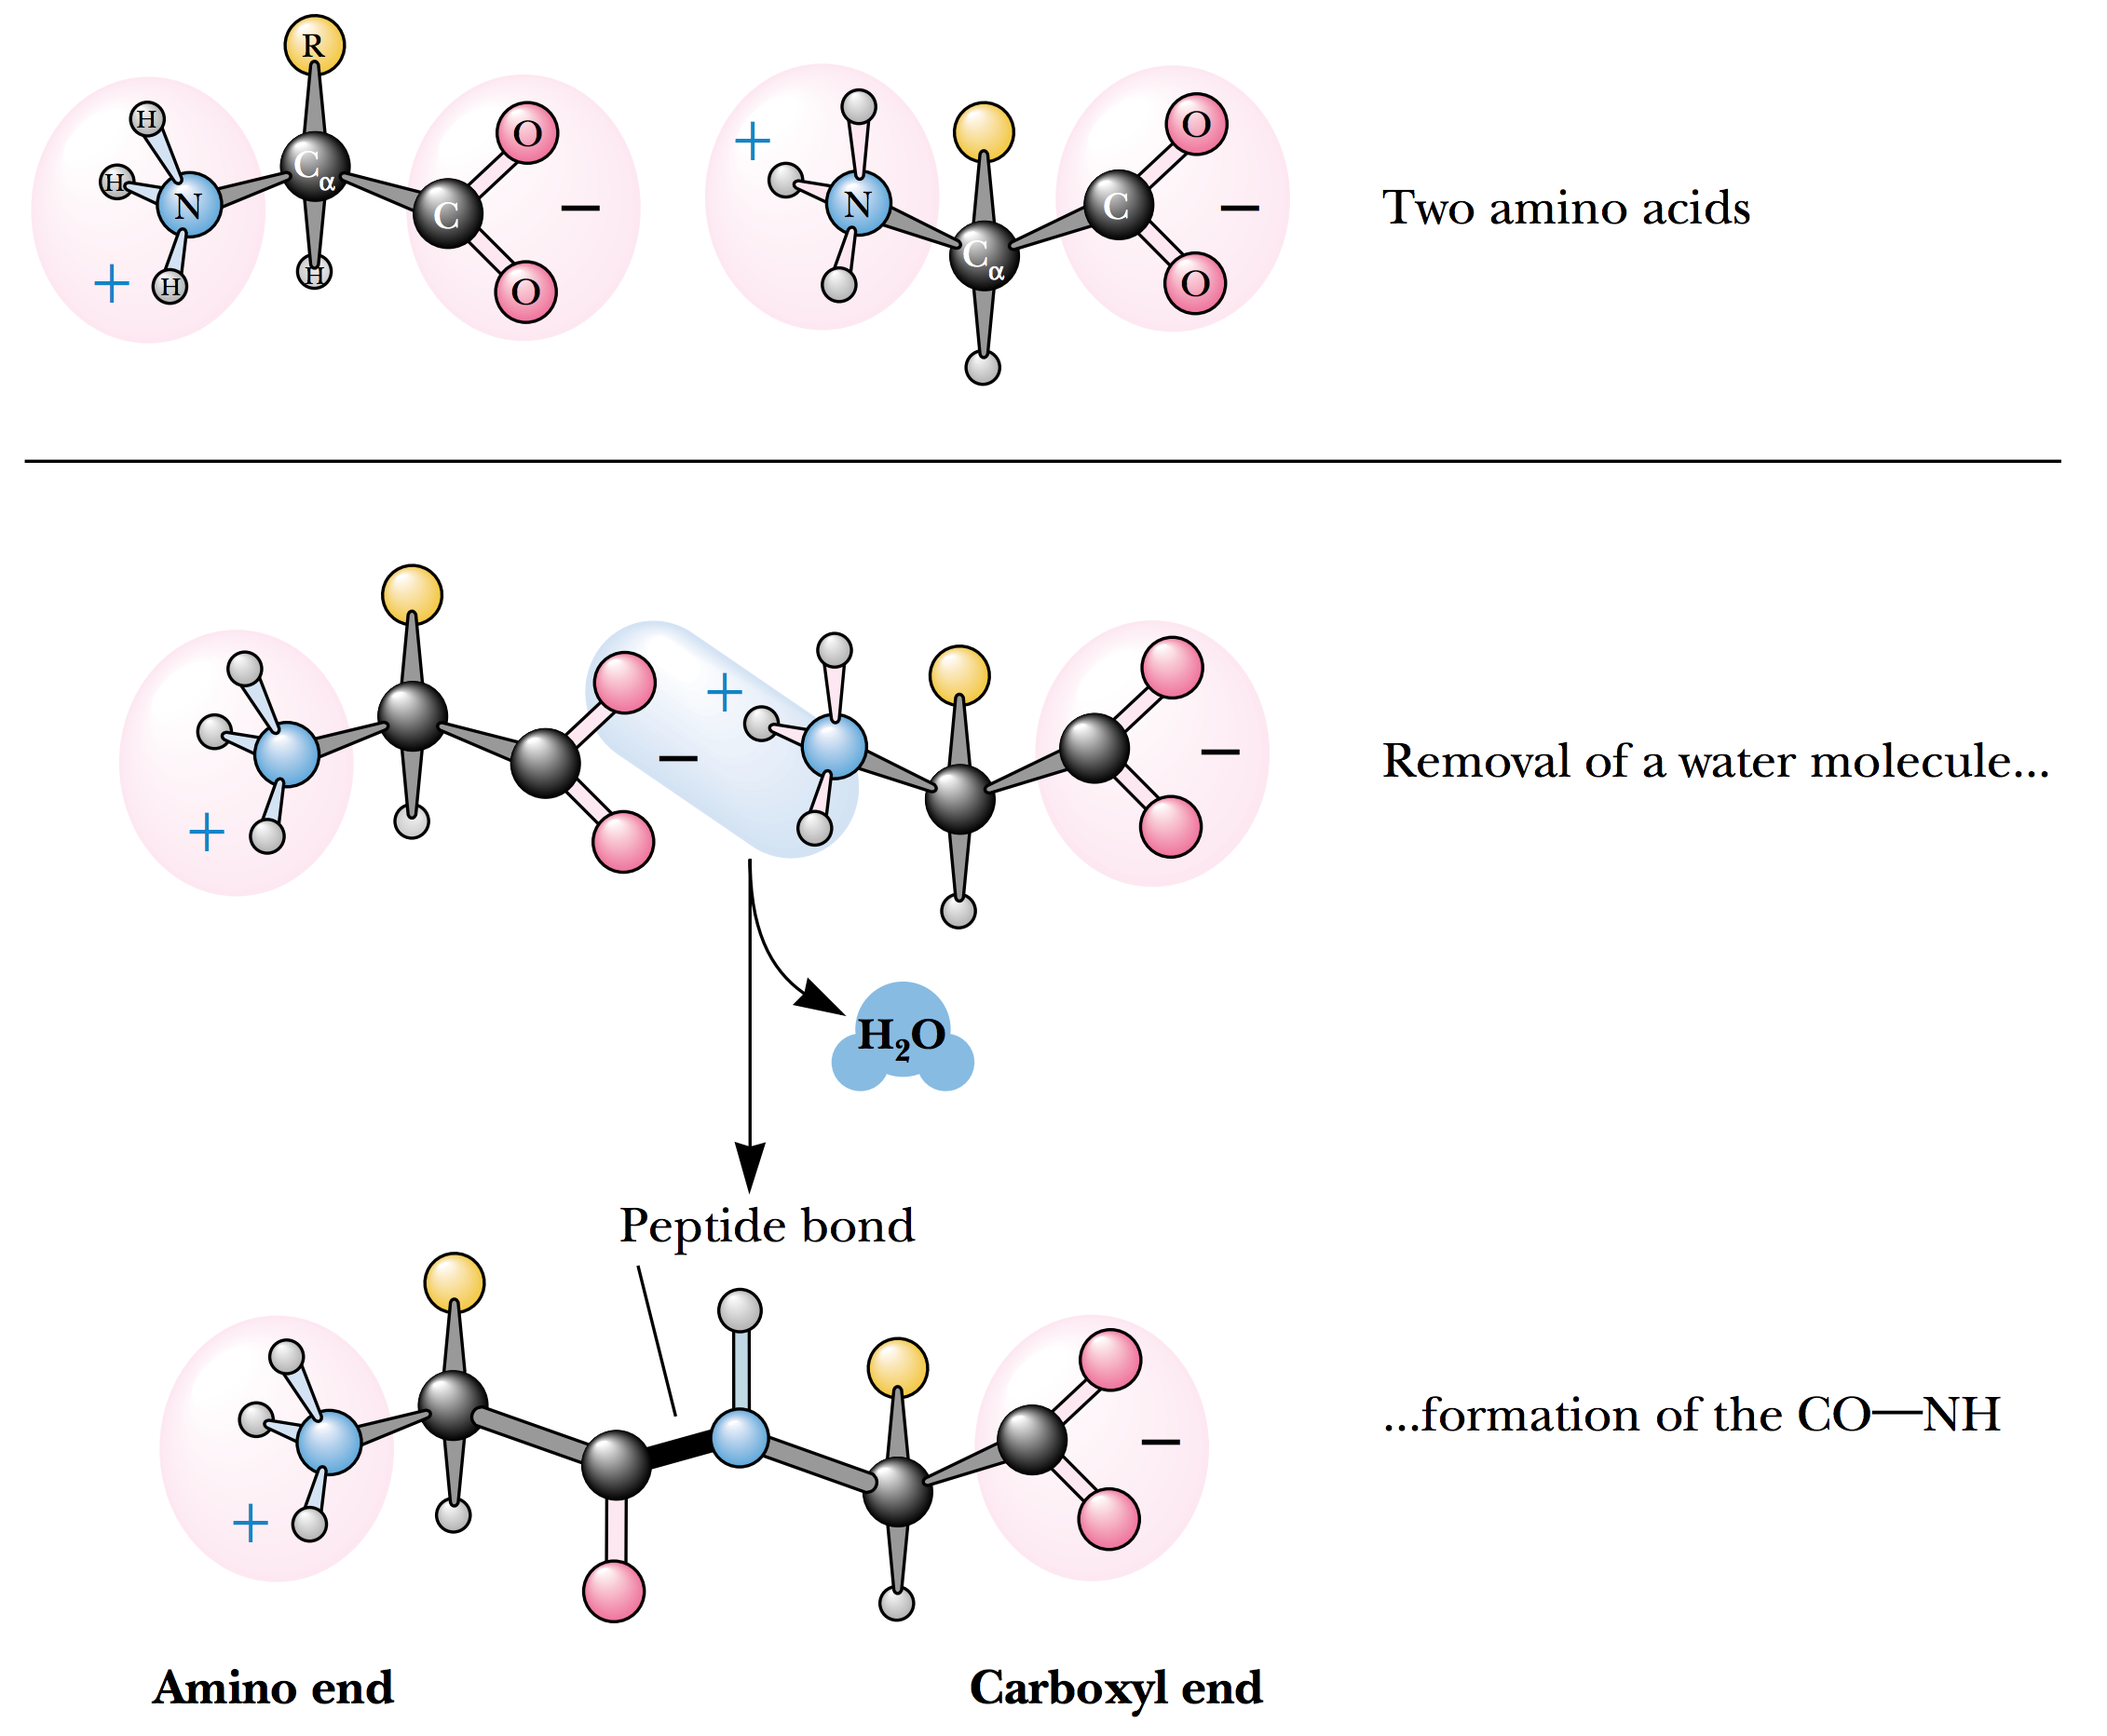
\includegraphics[width=\textwidth]{Figuras/peptide-bond.png}
    \caption{The Peptide Bond (Source: ~\cite{garrett1999biochemistry})}
    \label{fig:peptide-bond}
\end{figure}

When a peptide bond is formed and it starts to grow, it will assume a three
dimensional conformation. The manner in which the chain grows is directly
dependent on the dihedral angles that the peptide bond assumed. The dihedral
angles are enough to describe the protein to a high level of detail. The $N -
C_\alpha$ bound is described by the angle $\phi$. The $C_\alpha - C$ bound is
described by the angle $\psi$. Both the angles and $\phi$ and $\psi$ are
virtually free to rotate around its axis, limited only by steric clashes when a
part of the chain gets too close to itself. The $C - N$ pair is described by
the angle $\omega$. Due to complex interactions between the atoms in the chain
and its resonating properties, the $C - N$ bound behaves as if it was a double
bound. This limits the potential angles that $\omega$ can assume to regions
close to $0^{\circ}$ and $180^{\circ}$. The position where each dihedral angle
operates is shown on
Figure~\ref{fig:angles}.

\begin{figure}
    \centering
    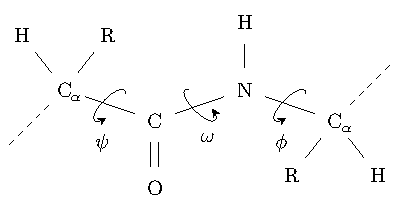
\includegraphics[width=0.7\linewidth]{Figuras/angles.pdf}
    \caption{Dihedral angles of an amino acid (Source: Author)}
    \label{fig:angles}
\end{figure}

The sequence of bonds $N - C_\alpha$, $C_\alpha - C$ and $C - N$ is called the
backbone. This chain extends over all the protein and is responsible for the
shape that it assumes, along with its interactions with the side chains. Due to
the constraints for $\omega$, the $N, C_\alpha, H$ and $O$ atoms will tend to
be co-planar. Two possible configurations are possible, the \textit{cis} and
\textit{trans}. In the \textit{cis} configuration the $\omega$ angle will be
approximately $180^\circ$ and the side chains will have alternate sides after
each peptide bond. This configuration is the most stable one. For the
\textit{trans} configuration, which a $\omega$ angle of $0^\circ$, the side
chains will be on the same side, making this configuration much less stable and
consequently less frequent.

While the tuple $(\phi, \psi, \omega)$ of dihedral angles is enough to
accurately describe the backbone, it lacks information about the side chains.
Due to the nature of the side chains, different side chains will have different
dihedral angles. Table~\ref{tab:side-chain-angles} shows the amino acids and
the number of side chain angles required to describe it.

\begin{table}[]
    \centering
    \begin{tabular}{l|l} \hline \hline
        Amino Acid & Angles \\ \hline \hline
        GLY, ALA, PRO & N/A \\
        SER, CYS, THR, VAL & $\chi_1$ \\
        ILE, LEU, ASP, ASN, PHE, TYR, TRP & $\chi_1$, $\chi_2$ \\
        MET, GLU, GLN & $\chi_1$, $\chi_2$, $\chi_3$ \\
        LYS, ARG & $\chi_1$, $\chi_2$, $\chi_3$, $\chi_4$ \\
        \hline \hline
    \end{tabular}
    \caption{Side Chain Angles}
    \label{tab:side-chain-angles}
\end{table}

\subsection{Protein Structures}
\label{sec:protein-structures}
%What are primary, secondary, tertiary and quaternary structures

% Present the different levels of details of the proteins at micro and macro
% levels
The analysis of a protein happens on increasing levels of details. There are
four structures commonly used in proteomics to identify, study and describe a
given protein and its properties~\cite{tsai2003introduction}.

% Primary structure
The primary structure of a protein is determined by the chain of amino acids
that form it. This sequence is encoded on the \ac{DNA}, and after the protein
syntheses is complete it will be inside the protein. The primary structure is
unique for each protein and can be used to uniquely identify it. For instance,
the
\textit{Methionine-Enkephalin}\footnote{\url{https://www.rcsb.org/structure/1plw}}
(1PLW) is a very simple polypeptide formed by 5 amino acids: Tyrosine, Glycine,
Glycine, Phenylalanine and Methionine. Using the one letter notation, the
primary sequence can be presented as YGGFM. This one letter sequence of amino
acids is available on protein sequence databases, such as the UniProtKB
database\footnote{\url{https://www.uniprot.org/help/uniprotkb}}.

% Secondary
The secondary protein structure consists of local patterns occurring on the
protein conformation. These patterns are three dimensional and together they
are used to assemble the protein. There are 8 accepted protein secondary
structures: 3 types of helices, 2 types of sheets, turns, loops and
coils~\cite{geourjon1995sopma}.

% helices
The helices can be split into three types: $\alpha$-helix, $3_{10}$-helix and
$\pi$-helix. Helices are characterized for having the $i$-th amino acid bonded
to the $i+k$-th amino acid, for a sequence of several amino acids. This bond is
a hydrogen bond between the amino group of the $i$-th amino acid and the
carboxyl group of the $i+k$ amino acid. The values of $k$ vary from 3 to 5, and
they determine the type of helix.

The more common type of helix is the $\alpha$-helix, which has $k=4$. That is,
the amino group of an amino acid is bonded with a hydrogen bond to the carboxyl
group of the amino acid four positions (in the primary sequence) after. There
are approximately $3.6$ amino acids per $\alpha$-helix turn, as shown in
Figure~\ref{fig:alpha-helix}. The secondary chain of the amino acids in this
type of helix are located on the outside of the  helix. The amino acids inside
this type of helix will have torsion angles close to ($\phi$, $\psi$) = (-58,
-47). An $\alpha$-helix can have from only one turn (formed by 4 amino acids)
to more than thirty, such as the human keratin (4ZRY).

\begin{figure}
    \centering
    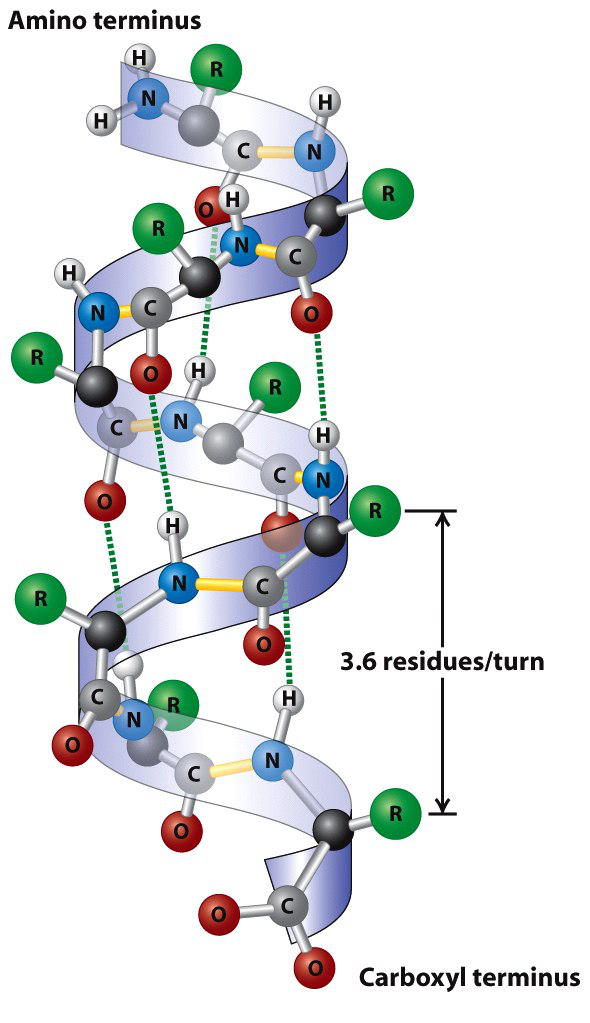
\includegraphics[width=0.5\textwidth]{Figuras/alpha-helix.jpeg}
    \caption{An $\alpha$-helix (Source:~\cite{lodish2008molecular})}
    \label{fig:alpha-helix}
\end{figure}

A seldom found type of helix is the $3_{10}$-helix. For this type of helix the
amino acids are bonded to the amino acid three positions after. This implies in
a helix more densely packed, and thus, less stable. Each turn has $3$ amino
acids and the torsion angles are around (-74, -4). A rarer type of helix is the
$\pi$-helix, where the hydrogen bonds happens 5 amino acids apart. There, each
turn as approximately 4.6 amino acids and the torsion angles are (-57, -70).
Accordingly to~\cite{borguesan2015apl}, $\alpha$-helix happens 34.1\% of the
time, $3_{10}$-helix less than 1\% of the time and $\pi$-helix about 4\% of the
time. Together, the three types of helix makes up for 39.1\% of the secondary
structures.

% Sheets
Another group of secondary structures are the sheets. They are characterized
for mainly for having planar surfaces. There are two types of sheets:
$\beta$-strands and $\beta$-sheets. The $\beta$-strands are sequence of usually
$3$ to $10$ amino acids with torsion angles of (-135, 135). $\beta$-strands and
$\beta$-sheets compose 25.2\% and 1.3\% of the secondary structures.

The $\beta$-sheets are formed from 2 or more $\beta$-strands, where each strand
bonds the adjacent ones. This bond is a hydrogen bond between the amino and
carboxyl groups of the amino acids, which happens in a alternating manner.
There are 2 types of $\beta$-sheets: Parallel and Anti Parallel. In the
parallel $\beta$-sheets all chains run in the same direction, as seem in
Figure~\ref{fig:parallel-beta-sheet}. In the anti parallel $\beta$-sheet the
chains runs in oposite directions, as represented in
Figure~\ref{fig:anti-parallel-beta-sheet}.

\begin{figure}[htbp]
    \centering
    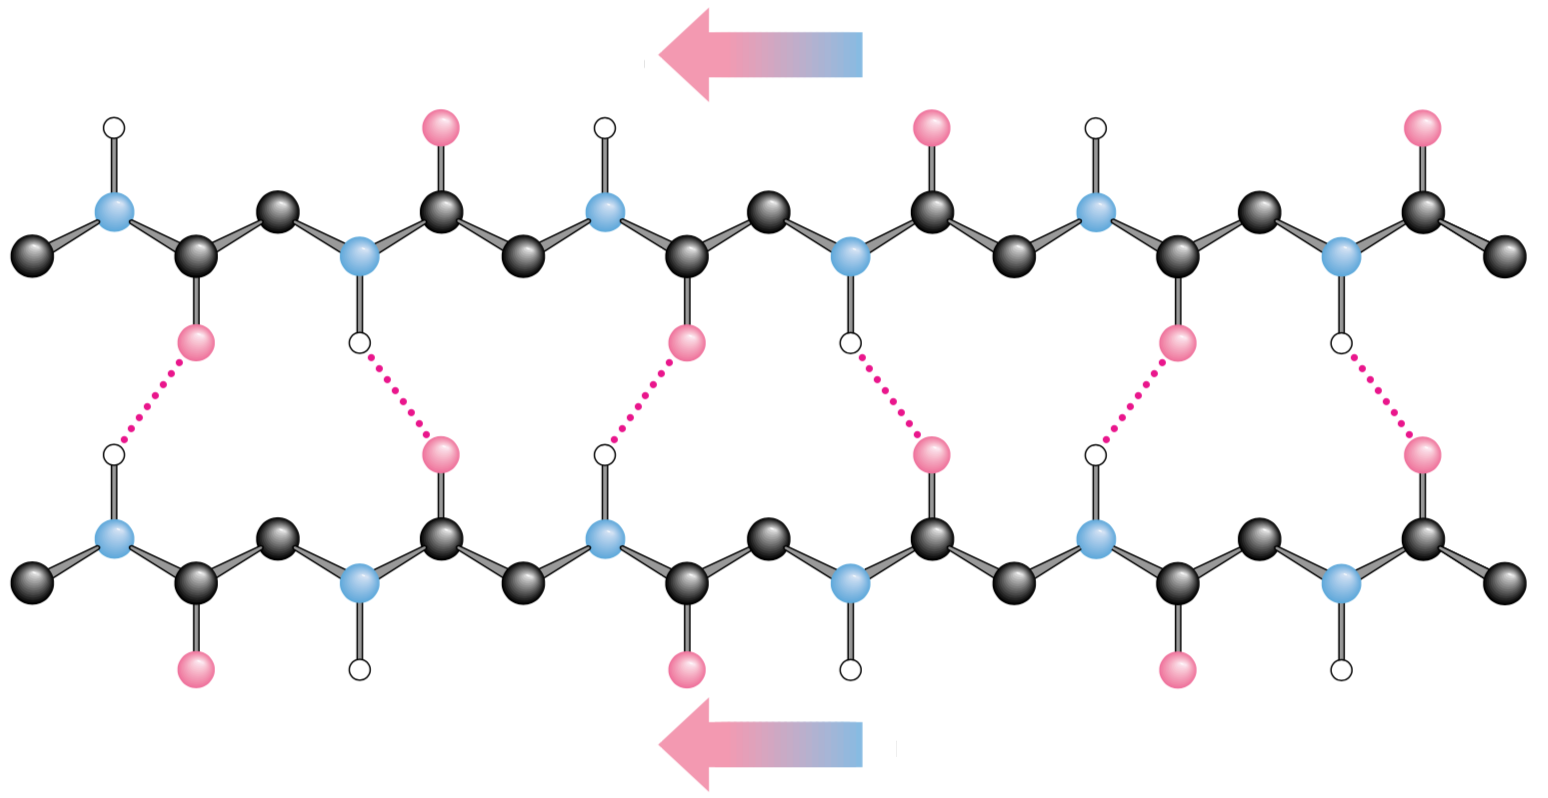
\includegraphics[width=0.5\textwidth]{Figuras/parallel-beta-sheet.png}
    \caption{A parallel $\beta$-sheet (Source: ~\cite{garrett1999biochemistry})}
    \label{fig:parallel-beta-sheet}
\end{figure}

\begin{figure}[htbp]
    \centering
    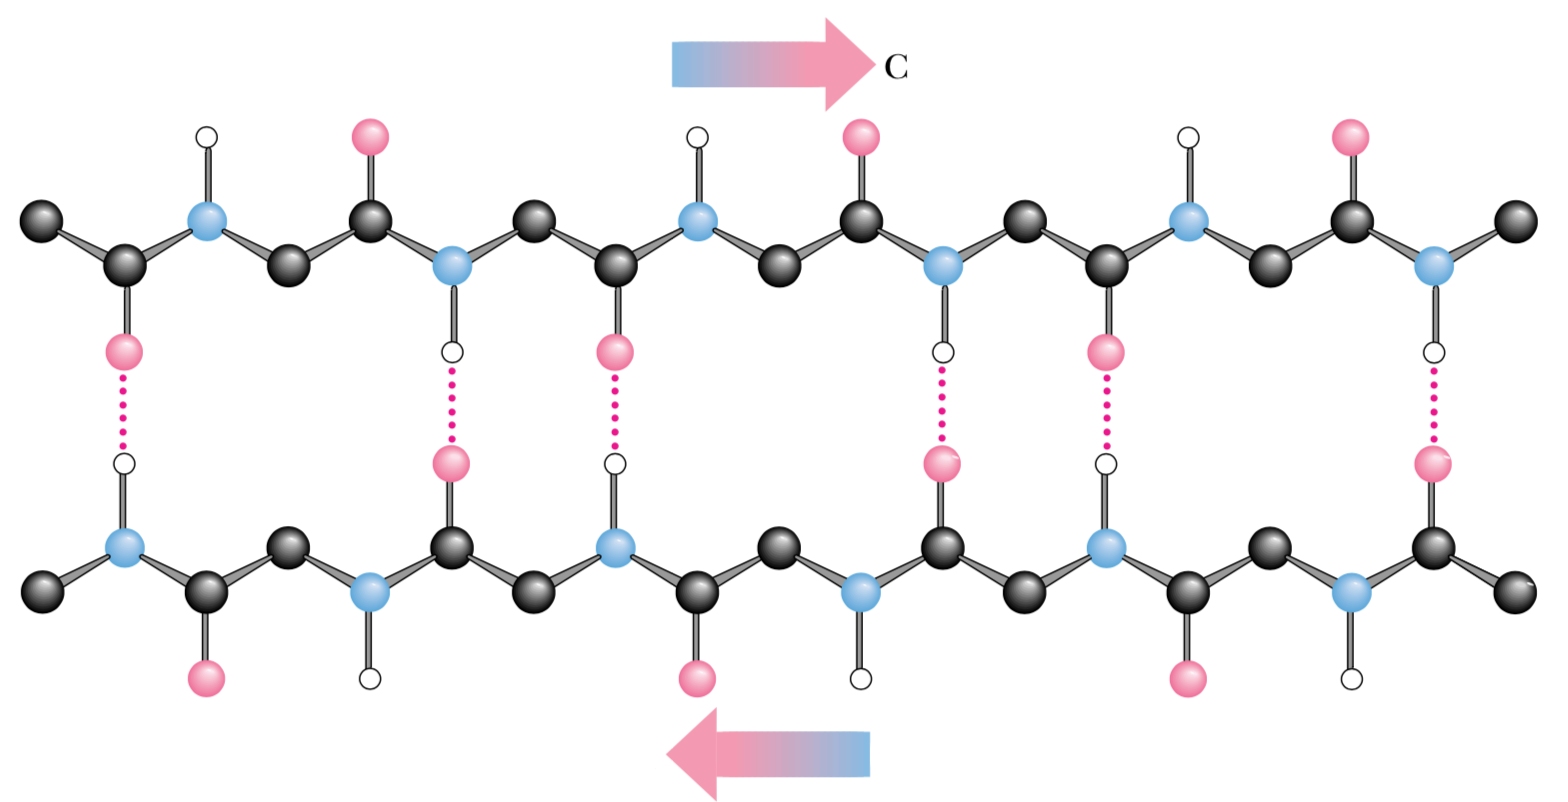
\includegraphics[width=0.5\textwidth]{Figuras/anti-parallel-beta-sheet.png}
    \caption{An anti-parallel $\beta$-sheet (Source: ~\cite{garrett1999biochemistry})}
    \label{fig:anti-parallel-beta-sheet}
\end{figure}

It is also possible for more than two $\beta$-strands to align forming a bigger
structure, called pleated sheets. In this structures, several $\beta$-strands
of the same alignment (parallel/anti-parallel) run along each other. This
allows for a $\beta$-strand to connect with the two neighbor $\beta$-strands.
An example of a anti-parallel pleated sheet in shown in
Figure~\ref{fig:pleated-sheet}. It is also possible that the ends of the sheet
bond to each other while being off-set by a single bond, thus making a shape
than resembles a cylinder.

\begin{figure}[htpb]
    \centering
    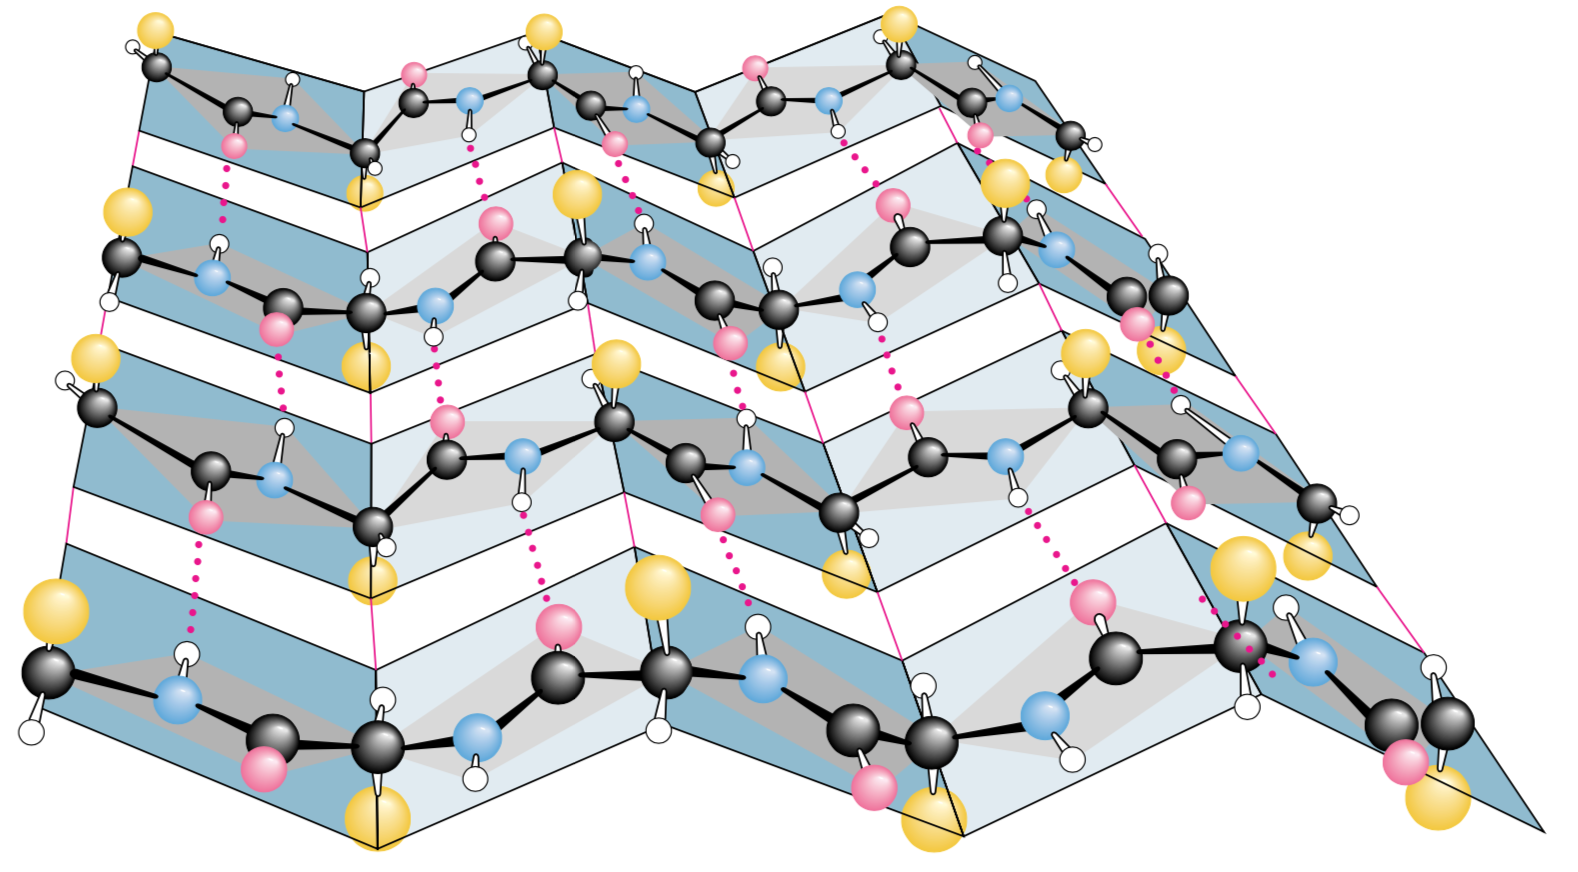
\includegraphics[width=0.75\textwidth]{Figuras/pleated-sheet.png}
    \caption{An anti-parallel pleated-sheet (Source: ~\cite{garrett1999biochemistry})}
    \label{fig:pleated-sheet}
\end{figure}

% other stuff (coils, turns and loops)
Finally, when there are no recurrent patterns on the secondary structure, it
can be either a loop, turn or a coil. A loop is a sequence of amino acids that
holds two helix or $\beta$-sheets together. If a loop is short and makes a
quick $180^\circ$ it is called a turn. If the amino acid sequence is located at
the start or the end of a protein, then it is called a coil. Turns and loops
represent 19.1\% of the secondary structures while coils represent 16.3\%.

% Tertiary
The tertiary structure is the three dimensional configuration of the amino
acids of a given protein. It can be also referenced as the native conformation.
The tertiary structure of a protein is directly dependant on the primary
structure. Also, the functionality of the protein is dependent on the tertiary
structure. A fact that rises the importance of being able to determine the
native conformation of a protein.

While the secondary structure references amino acids only locally, on the
tertiary structure all amino acids are relevant to the final structure.
Figure~\ref{fig:1ctf} shows a ribosomal protein of the Escherichia Coli
(1CTF)\footnote{http://www.rcsb.org/structure/1CTF} composed by 74 residues.
The figure shows the native conformation of the protein, i.e. its tertiary
structure. It also shows grouped in colors the secondary structures. The
$\alpha$-helices are presented in pink, $\beta$-sheets are presented in yellow
and white denotes coils. The combination of the secondary structures assemble
the tertiary structure. Furthermore, the tertiary structure describes how each
secondary structure relates to each other.

\begin{figure}[htbp]
    \centering
    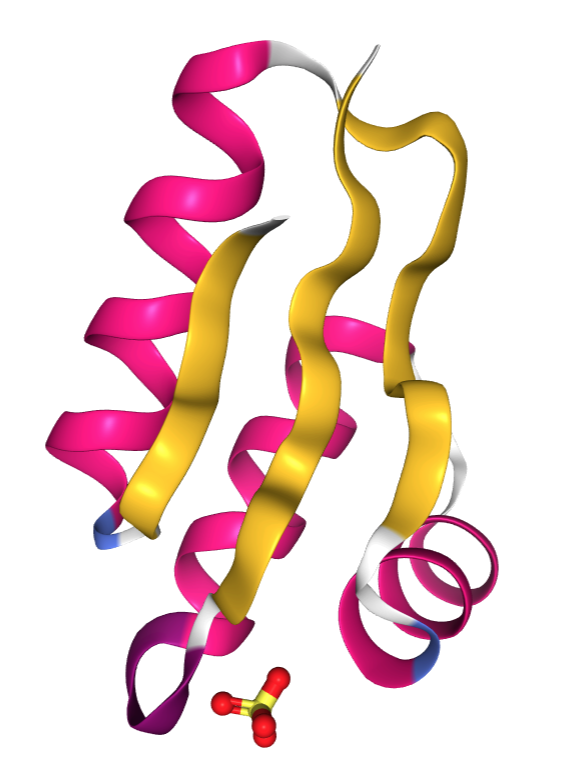
\includegraphics[angle=90,origin=c,width=0.6\textwidth]{Figuras/1ctf.png}
    \caption{The native conformation of protein 1CTF (Source: RCSB PDB)}
    \label{fig:1ctf}
\end{figure}

% Levintal's paradox describes a seemingly paradoxical situation where the protein

% Quaternary
There are certain groups of proteins that on its own are not able to exercise
its function. They need to be combined in pairs or even in bigger numbers. This
agglomeration of proteins is the quaternary structure, present in some (groups
of) proteins. A well know protein with a quaternary structure is the human
hemoglobin (1A3N)\footnote{\url{https://www.rcsb.org/structure/1a3n}}, formed
by 4 proteins. Figure~\ref{fig:human-hemoglobin} shows the assembly of four
proteins, the green point at the center shows a point of rotational symmetry
between the proteins.

\begin{figure}
    \centering
    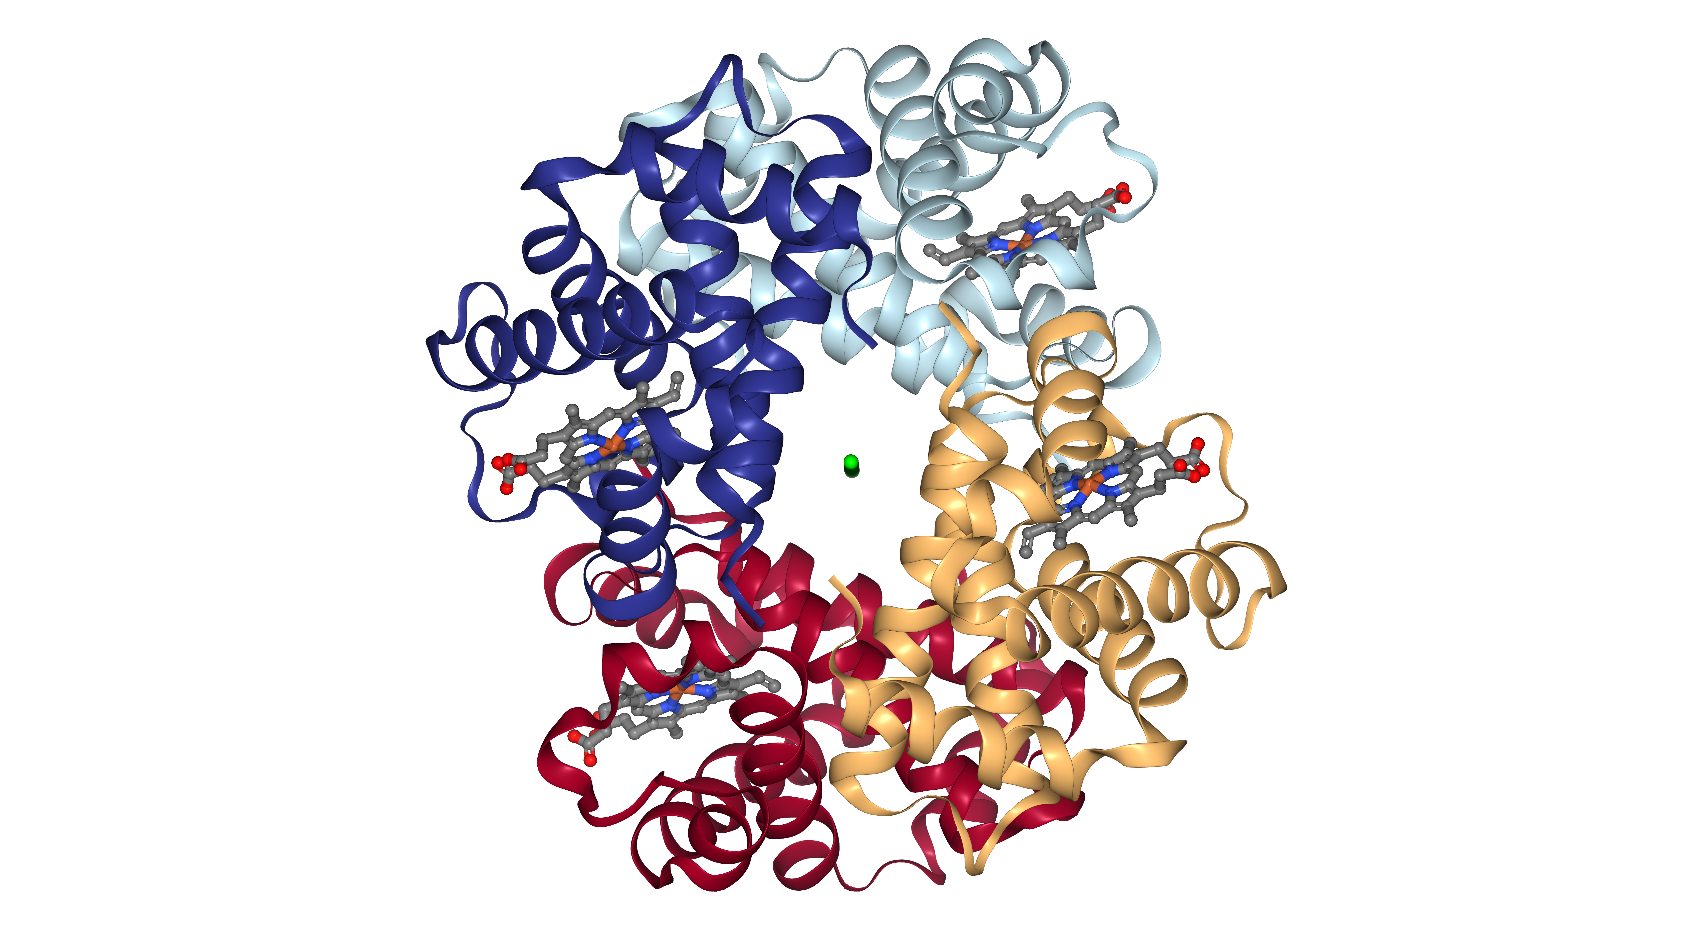
\includegraphics[width=0.6\textwidth]{Figuras/1a3n.png}
    \caption{The quaternary structure of the hemoglobin. Each color denotes one protein chain. The green point in the middle marks the point of radial symmetry. (Source: RCSB PDB)}
    \label{fig:human-hemoglobin}
\end{figure}

\subsection{Protein Secondary Structure Prediction}
\label{sec:secondary-structure-prediction}
%Secondary protein structure prediction problem

As previous shown on Section \ref{sec:protein-structures}, the secondary
structure plays a significant role in describing the native conformation of a
given protein. While not enough on its on, knowing in advance the secondary
structure of a protein allows one to work on how the groups of amino acids in
each substructure relates to each other instead of having to figure out how all
amino acids relates to each other. Therefore, knowing, even only approximately,
the secondary structure of a protein is a very important asset during the
process of predicting the tertiary structure.
background
Currently, there is no \textit{in vitro} method of determining only the
secondary structures of a protein. However, it is possible to employ
mathematical and computational methods. Considering that some amino acids have
more propensity of forming certain secondary structures, it is possible to
conduct an statistical analysis in order to assess the likelihood of an amino
acid forming a particular structure. This kind of analysis has been done
in~\cite{dunbrack1993backbone} and~\cite{borguesan2015apl}.

Given the number of proteins with a known structure, it is possible to use data
mining and artificial intelligence methods for predicting the secondary
structure. This approach is the more explored one so far.
In~\cite{wang2016protein} the authors used deep neural networks for predicting
the secondary structure. Feed forward neural networks were used
in~\cite{meng2016computational}. In~\cite{kathuria2018predicting} the authors
employed random forests to predict the secondary structure.
In~\cite{baldi1999exploiting} the authors used recurrent neural networks.
In~\cite{kim2018dihedral} the use of generative adversarial networks was
explored to predict the dihedral angles of the secondary structures.
In~\cite{pollastri2002improving} and~\cite{mcguffin2000psipred} the authors
used the output of (multiple) sequence alignment algorithms as the input of
simple feed forward neural networks. These two implementation were ranked top
in the \ac{CASP}~\cite{moult1999critical} and are still largely used to this
date. More details on secondary structure prediction are available
in~\cite{jiang2017protein}.


\section{Protein Structure Prediction}
\label{sec:psp}
\label{sec:pspp}
\label{sec:protein-structure}

%In contrast to the methods presented in Section~\ref{sec:protein-structure},
%\textit{in silico} methods required only information that is more easily and
%fastly obtainable. At this point, however, they are not viable for larger
%(more than 100 amino acids) proteins. Nevertheless, a significant effort has
%been put into improving the current methods.

%In this section it is presented topics on protein computational
%representation, on and off lattice models and the main prediction methods are
%presented as well.

%\subsection{Protein Representation} \label{sec:protein-representation} on and
%off lattice

In a laboratory environment, i.e. \textit{in vitro}, it is possible to
determine the native conformation of a given protein using mainly two methods.
The first method is know as X-Rays crystallography~\cite{nelson2008lehninger}.
Overall, the X-Ray crystallography has a better quality in the data generated,
however, it can only work on crystallized structures. Due to this fact, it is
possible that during the process of crystallization of a given protein sample
it crystallizes in a conformation that is not exactly its native one. Proteins
\textit{in natura} are dynamic molecules, that can vibrate and tumble around.
This property is lost when using X-Ray crystallography.

The other more recent method is ~\ac{NMR}~\cite{nelson2008lehninger}. This
method has a slighter lesser accuracy, however, it can work with proteins in an
aqueous environment. Thus, having a trade off that can offset the downsides of
X-Ray crystallography. Nevertheless, both methods are error prone, possibly
outputting noisy data. They also are expensive and take a considerable human
effort and economic resources to be utilized.  Thus the need for a \textit{in
silico} method of determining/predicting the protein structure.

The process of predicting the structure of a protein requires that it be
represented computationally in some way. The folding process \textit{in natura}
happens very fast, spontaneously and in a continuous environment. However, in
order to represent the protein computationally, some trade off is required
between level of detail and processing power required. Arguably the main
division between the models are the on lattice models and the off lattice
models.

The on lattice model, as the name implies, are models where the structures are
constrained to a lattice. Possibly the simplest model is the 2D \ac{HP} Model.
It is composed of points representing the amino acids, which can be either
hydrophobic or polar and are constrained to a 2D quadrilateral lattice. Despite
its simplicity, this model is already
$\mathcal{NP}$-complete~\cite{berger1998protein}. A 3D approach to a \ac{FCC}
lattice is presented in~\cite{hoque2007protein}, which also is a
$\mathcal{NP}$-complete problem. A triangular lattice approach is studied
in~\cite{agarwala1997local} in two and three dimensions. At the time of the
publication it was not know if that particular model was a
$\mathcal{NP}$-complete problem, latter it was proved to be. In fact, as
demonstrated by~\cite{hart1997robust}, the protein structure prediction problem
is $\mathcal{NP}$-complete regardless of the lattice used to represent it.

% explain off lattice models
Despite the on lattice model simplicity, it still is an intractable problem on
large scale due to its $\mathcal{NP}$-completeness. Furthermore, from a
practical point of view, these models can not represent a protein with enough
details to be able to replace an \textit{in vitro} method for determining the
protein structure. Therefore, a more robust representation is required. This
higher representation power is possible using off lattice models, that is, a
model that is not constrained by a lattice.

What can possible be considered the simplest model is the AB Off lattice model,
which represents the amino acids as spheres that are either hydrophobic or
polar, and the angles between them are not
constrained~\cite{berger1998protein}.  A more detailed model consists of using
the coordinates of the $C_\alpha$. In this model the amino acids are abstracted
into spheres, however, they maintain their properties such as polarity and
hydrophobicity, allowing for a increased level of detail. It is possible to
represent each of the amino acid heavy atoms (Nitrogen, Carbon and Oxygen)
individually, instead of using an sphere to represent the whole amino acid.
This model allows for interactions between individual atoms in the  backbone to
be considered during the prediction.

Evolving even more the level of detail, it is possible to represent all atoms
in the backbone, including the Hydrogen atoms. This permits that hydrogen bonds
be taken into account, which plays a significant role in the formation of
secondary structures and in the interactions between them. Furthermore, it is
possible to include an ellipsoid (also called centroid) to describe the amino
acid side chain. With this, the shape of each amino acid also can be considered
when predicting the three dimensional structure of the protein.

To fully represent the protein, there are two main models. Backbone and side
chain torsion angles and all atoms coordinates~\cite{rohl2004protein}.  The
former describes all atoms in the protein, including the side chain. However,
the bond length between these atoms are fixed as well as the position of the
hydrogen atoms. This model is enough to describe the protein very accurately
and to take into account most of its interactions. Nevertheless, since
artificial constrains are imposed in the model, it is possible that some
proteins can not be correctly predicted because it depends on one of the
aspects that the model removed. For this reason the all atom coordinates model
can be employed. In this model all atoms are considered and have all their
degrees of freedom. Currently, this model is the most accurate one, at the
expense of adding up a hundred variables per amino acid.

\subsection{Ab Initio Methods}\label{sec:ab-initio}

One of the main class of protein prediction algorithms are the ab initio
methods~\cite{lee2017ab}. From the Latin, ab initio means \textit{first
principles}. These methods are called as such because they work based only on a
primordial aspect of the proteins: They are physicochemical objects. And as
such, they follow well know rules.

The information about the physical and chemical properties from the proteins
are encoded on the protein representation as discussed on
Section~\ref{sec:pspp}. Its interactions are evaluated by energy functions (or
scoring functions). A given protein \textit{in natura} seeks its point of least
potential energy~\cite{anfinsen1973principles}. Based on this fact, an energy
function for an \textit{ab initio} method tries to evaluate the potential
energy of a given conformation. Then, with a search procedure it is
(theoretically) possible to find its point of least potential energy, which
should be at least close to its respective native conformation. In other words,
\textit{ab initio} methods can be seem as an optimization problem where the
objective function is the energy function of the protein and its variables are
the degrees of freedom from its computational representation.

% present some energy functions
There are several energy functions in the literature which allows for an
\textit{ab initio} approach, such as the \ac{AMBER}, \ac{GROMOS}, \ac{CHARMM} e
Rosetta.  The \ac{AMBER}~\cite{salomon2013overview} package contains a set of
scoring functions based only on the potential energy of proteins (and other
molecules). Its original use was intended for molecular dynamics simulations.
However, its is possible to use it just to score a given conformation. Another
package which offers energy functions for proteins is
\ac{CHARMM}~\cite{brooks2009charmm}. Similar to \ac{AMBER}, it is also
primarily intended for molecular dynamics simulations for several organic
molecules of interest. Nevertheless, its scoring can be used for \textit{ab
initio} methods. The \ac{GROMOS} package~\cite{eichenberger2011gromos++} also
intended for molecular dynamics simulations can provide energy scoring of
protein conformations. A more detailed discussion of the energy functions is
available at~\cite{dorn2014three}. In~\cite{narloch2016diversification}
explored the differences between \ac{AMBER}, \ac{CHARMM} and Rosetta. A further
discussion on energy fields (from molecular dynamic packages) can be found
in~\cite{vlachakis2014current}.

Several energy functions are used in the literature. The Rosetta
suite~\cite{rohl2004protein,kaufmann2010practically} contains multiple energy
functions for all atom coordinates models, backbone and side chain torsion
angles and backbone torsion angles with centroids for the side chains. This
suite also allows for the customization and creation of new energy functions.
The energy functions there consider both the physicochemical properties of the
protein as well as its statistical nature, based on a knowledge database with
propensities of each amino acids. Information regarding the compactness of the
structure and other properties such as the formation of side chain structures
are also computed. This removes the possibility of scoring the protein with an
physical unit of measurement. Instead, the energy functions are measured by the
\ac{REU}. More information about the information considered is available
in~\cite{alford2017rosetta}.

% Briefly present the optimizers
With an energy function for scoring the protein conformations, it is possible
to employ an optimizer in order to search for an conformation of least
potential energy. This procedure must sample the conformation space accessible
from the computational representation of a given protein. A vast range of
methods has been employed over the years in the literature.
In~\cite{li1987monte} a Monte Carlo based search is used to optimize a set of
dihedral angles. Basin-hopping is a method where a random perturbation is
applied to the conformation and then a hill-climbing type of algorithm is
employed to find a local minima. It has been used in~\cite{prentiss2008protein}
and~\cite{olson2012efficient}.

One particular branch of algorithms that have been used extensively in the
literature are bio inspired algorithms. The more well established algorithms
are present in the literature, such as the \ac{PSO}~\cite{geng2017protein},
\ac{DE}~\cite{hao2017conformational} and the \ac{GA}~\cite{higgs2010genetic}.
Other algorithms that are not so widely used have been also explored for the
\ac{PSPP} such as the Cuckoo Search (CS)~\cite{ramyachitra2017modcsa} and the
Bee Colony Algorithm~\cite{li2015balance}. This topic is explored in further
detail in Section~\ref{sec:bioinspired}.

\subsubsection{The Rosetta Suite} \label{sec:rosetta}

Practically, working with an \textit{ab initio} method is very time consuming,
due to the high amount of boilerplate code required to be able to model the
protein and its molecular dynamics from scratch. Furthermore, this process is
also very error prone. The Rosetta Suite~\cite{rohl2004protein} introduces a
robust and validated suite for working with proteins and other macromolecules.
It also includes multiple utilities for manipulating, pre-processing and
post-processing the protein conformations in a pipeline. The Rosetta Suite is
free for academic use, open-source and is available at
\url{https://www.rosettacommons.org/}.

One of the tools available at Rosetta and required for this work is fragment
insertion. A fragment consists of a sequence of continuous amino acids at a
specific configuration extracted from some protein of known structure. This
sequence must fully match to some continuous sequence of amino acids in the
target protein, where the structure is not yet known. The purpose of this is to
use multiple fragments as building blocks. It is worth noting that fragments
from homologous structures are removed, as for to remove the potential sampling
from the same protein from another organism for example.

The process of creating a set of fragments for a particular target protein
is required to be run only once per target and per fragment size. Two sizes of
fragments commonly used are 3 and 9. So if a fragment set is being created
for a given target protein, then the fragment picker must be run twice. The
fragment picker is the module responsible by searching a database of
non redundant protein conformations and sampling it in order to assemble
fragments. More information about the inner workings of the Rosetta Fragment
Picker is available at~\cite{gront2011generalized}.

Rosetta includes two fragment insertion operators (called \textit{movers} in
Rosetta). One is the classical\footnote{Found in Rosetta as
ClassicFragmentInsertion} fragment insertion and the other operator is the
smooth\footnote{Found in Rosetta as SmoothFragmentInsertion} fragment
insertion. The classical operator simply replaces one portion of the protein
with its respective fragment. This change can be very aggressive and have a
high changing impact on the protein conformation. Due to the high impact of
this operator, there is a high chance that the operator will produce a
conformation with a worse energy score, and therefore be rejected if used under
a \ac{MC} search.

The smooth fragment insertion applies a classic fragment insertion followed by
a second fragment insertion that tries to minimize the Gunn
Cost~\cite{gunn1997sampling}. The Gunn Cost measures the amount of change in a
conformation due to the arm lever effect. That is, the further away from the
insertion point an amino acid is, the more it will move. Since the smooth
fragment insertion tends to negate some of the change it will preserve some of
the structure of the protein, leading to a more localized change in the
conformation. It is worth noting that the smooth fragment insertion is an
optimization problem as well, which minimizes the Gunn Cost.  Since this
operator tries to minimize the amount of change by its application, the impact
on the energy score will be smaller, leading to smaller and more refined
changes. This, under a \ac{MC} situation will potentially lead to a higher
acceptance rate.

\subsection{Knowledge Based Methods}

% Why use it
Due to the limitation that \textit{ab initio} methods currently have, other
methods have been utilized in the literature with greater success. These two
methods are the \ac{TM} Methods~\cite{dorn2014three} and \ac{HM}
Methods~\cite{leach2001molecular}. Contrary to the \textit{ab initio} methods,
these two methods require previous information to be available in order to be
successful.

%Threading
\ac{TM} assumes that protein structure is, to some degree, preserved during the
evolution of organisms. Therefore, proteins with a certain degree of difference
in the primary sequence may have a very similar tertiary structure. A set of
template proteins is used as to represent the conformation space. Then, the
amino acid sequence of the target and template protein are aligned in order to
fit the target protein into the template. Then, the model is refined and the
final prediction is then output. In the event of the target protein having the
same overall fold as the template, the prediction can achieve very high levels
of accuracy. However, if a suitable template can not be found, the prediction
will be of poor quality. This is one of the main downsides of the \ac{TM}
method. It requires a suitable template. Nevertheless, \ac{TM} has had the best
results in recent \ac{CASP} events~\cite{moult2018critical}.

%Homology
\ac{HM} is to an extent similar to \ac{TM}. However, while \ac{TM} relies on
potential evolutionary similarities between proteins, HM expects homologous
(similar primary sequence) to have similar tertiary structures. Thus, HM
depends on the existence of a protein with a sufficient degree of similarity.
If such protein exists (and has its native conformation available) then it is
possible to arrive a high degrees of accuracy.

% downsides
Both \ac{TM} HM require that a suitable known protein to exist to be used as
template. Either one with evolutionary similarity for \ac{TM} a homologous
protein for HM. If such proteins do exist, then these methods will have a very
high chance of outperforming \textit{ab initio} methods. However, as the degree
of similarity decays so does the performance of the method. At this point
\textit{ab initio} methods have a chance of outperforming knowledge based
methods.

\subsection{Evaluating Protein Errors}\label{sec:protein-metrics}

Regardless of the method being used for predicting the protein structure, in
order to conduct research in this area it is necessary to measure error in the
prediction. Error measurement has been an active sub area of research in the
\ac{PSP} field, with dozen of such metrics being proposed since the \ac{PSP}
started to grow in
interest~\cite{xu2010significant,zhang2005tm,siew2000maxsub}.  Different
metrics focus on different aspects of the prediction, and while they should be
somewhat directly correlated between then it is possible that different metrics
do not always agree on the quality of a prediction. Therefore, it is important
to know the metrics and how they can evaluate a prediction.

Currently, when conducting a research, the main way of measuring error is to
compare the predicted structure against the one that was found \textit{in
vitro}. With this, it is possible to measure how far (or close) a prediction is
from the ground truth. This approach, however, has some flaws. The main one is
that determining the protein structure \textit{in vitro} has an error margin.
That is, the native conformation found by \ac{NMR} and X-Rays crystallography
methods has a finite resolution, typically in the order
of 1 to 3 Angstroms. Due to that, getting and error too low is rather
pointless, since instead of measuring against the native conformation
it would be measuring against the method itself. Other point that is
worthwhile to take into account is that it may be required to have the
protein in a crystal form in order to study its conformation
\textit{in vitro}. Naturally, the proteins are in an aqueous environment,
surrounded by several substances. The crystallization process therefore
removes the protein from its natural environment and forces it in a
solid state~\cite{wuthrich1989protein}.
This also inserts some degree of error into the model. As it can be seen
on Figure~\ref{fig:protein-error}, 19 conformation samples obtained
\textit{in vitro} are superimposed and show a noticeable variation.
This variation occurs dues to the reasons listed above.

\begin{figure}
    \centering
    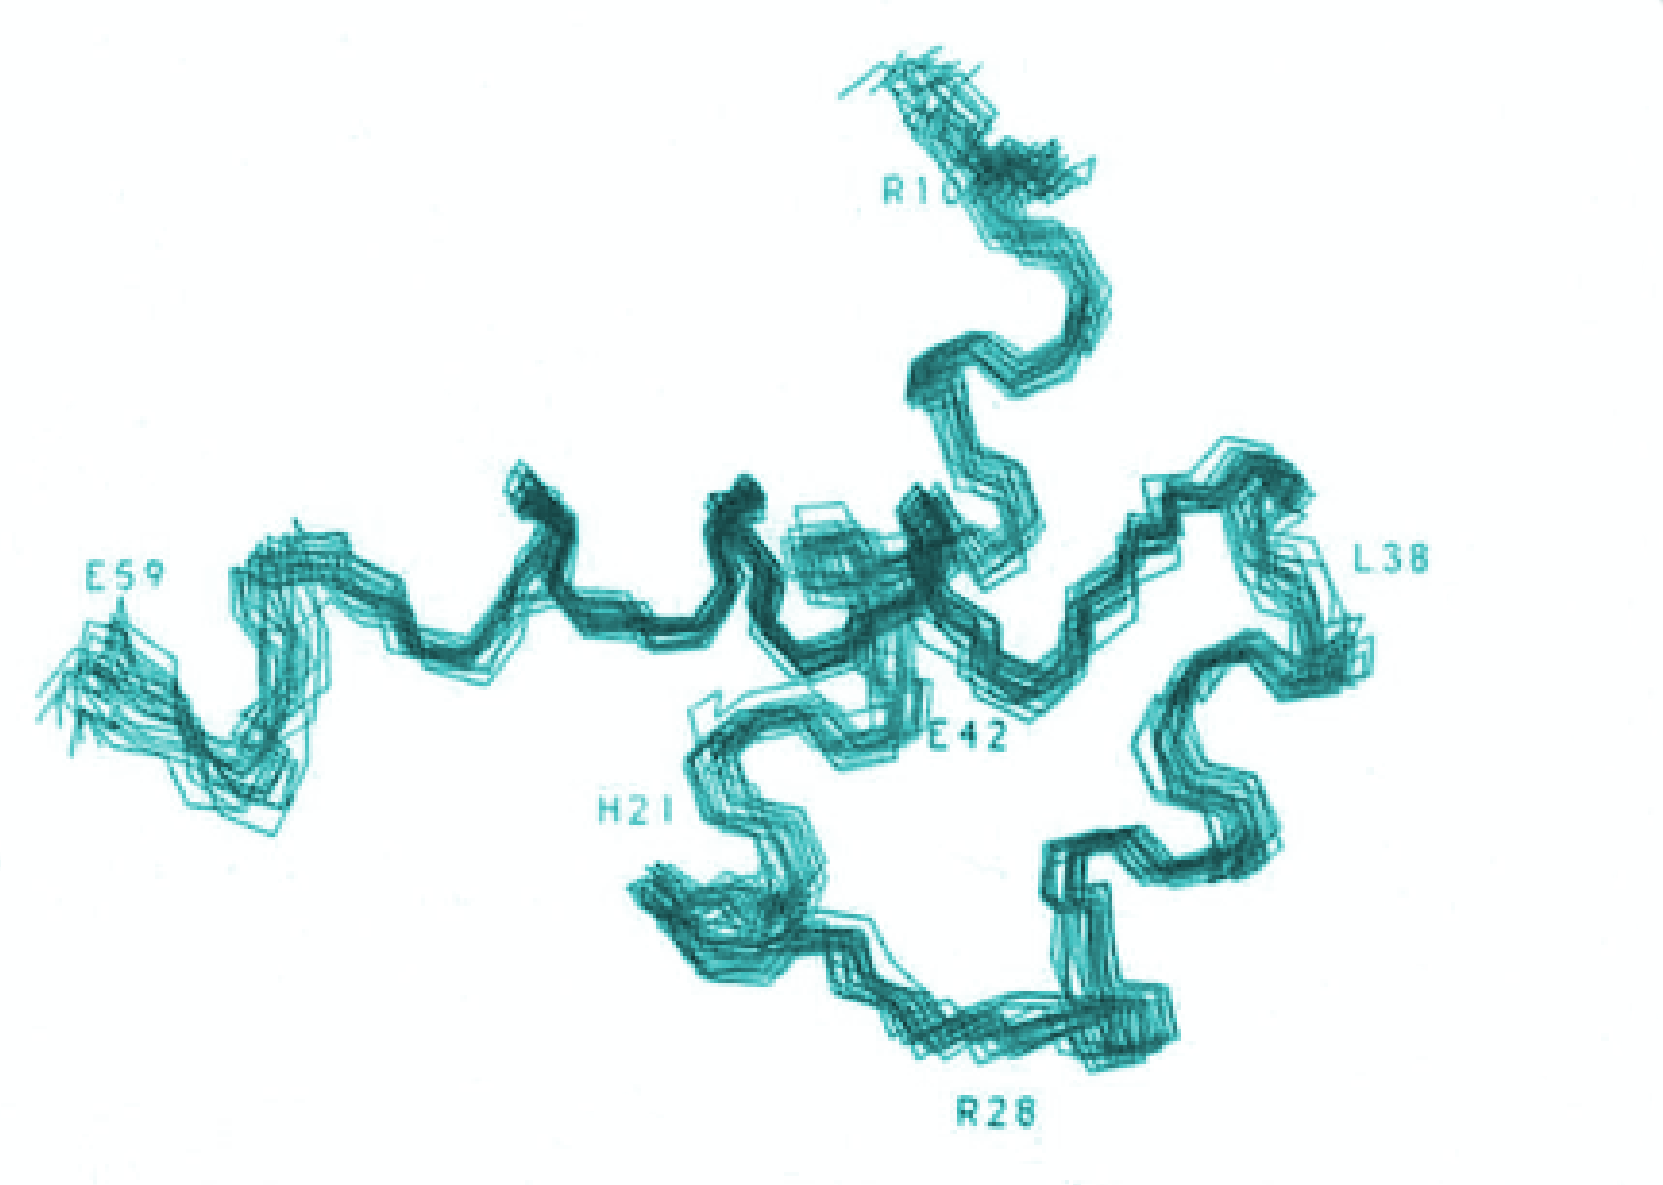
\includegraphics[width=0.7\linewidth]{Figuras/protein-error.png}
    \caption{19 aligned samples of a protein determined by \ac{NMR} (SOURCE (ADAPTED): \cite{wuthrich1989protein})}
    \label{fig:protein-error}
\end{figure}

Possibly the most well known protein prediction measuring method is the
\ac{RMSD}. It is typically applied to the alpha carbons, and thus only
measuring the error in the backbone. However, it can also be applied to all
atoms in the protein. The formula for the \ac{RMSD} is shown in
Equation~\eqref{eq:rmsd}. As the name suggests, the \ac{RMSD} is calculated as
the Square Root of the mean from the squared deviation.

\begin{equation} RMSD (A, B) = \sqrt[2]{\frac{\sum^{n}_{i = 1}{(A_i -
B_i)^2}}{n}} \label{eq:rmsd} \end{equation}

The fact that the deviation is squared and averaged leads to some downsides in
this measurement method. Firstly, a bigger protein can have a much higher error
due to the deviations being squared over the number of atoms being considered.
This makes the comparison of prediction quality between different proteins
impractical. For example, an error of $4{\AA}$ in a 50 residue protein is
different from $4{\AA}$ in a 150 residue protein. Furthermore, since the
deviation is squared, small deviations in some keys places of the conformation
will lead to an error that propagates over the protein due to an arm lever
effect.

In order to avoid the downsides of the \ac{RMSD}, several other metrics have
been proposed. Two of them saw great use in \ac{CASP}~\cite{moult2018critical}:
\ac{GDT-TS}~\cite{zemla2003lga} and the \ac{TM-Score}~\cite{zhang2004scoring}.
\ac{GDT-TS}, meaning Global Distance Test-Total Score is a measurement which
considers four successive alignments and is shown in Equation \ref{eq:gdt-ts}.
Each alignment uses a cutoff from $1{\AA}$ to $8{\AA}$ going in powers of two.
The score consists of the mean of the ration of the maximum number of atoms
that can be aligned using there cutoffs. It is worth noting that calculating
the \ac{GDT-TS} is a $\mathcal{NP}$-Hard problem on its own. Nevertheless,
heuristics that are sufficiently fast and accurate have been developed to make
it of practical use.

\begin{equation} \text{GDT-TS} = ( GDT_1 + GDT_2 + GDT_4 + GDT_8 ) / 4
\label{eq:gdt-ts} \end{equation}

The \ac{TM-Score} can be considered an extension of the \ac{GDT-TS}. While
\ac{GDT-TS} improves upon \ac{RMSD}, it has some downsides of its own. For
instance, the fixed thresholds may lead to semantic differences when
considering proteins of different sizes. That is, a smaller protein will be
able to fit more atoms inside the threshold more easily than a bigger protein,
thus rendering the measurement method somewhat dependent on residue length,
even though the score is normalized between 0 and 1.

\ac{TM-Score} aims to provide a dynamic threshold value based on the protein
length, and with this, provide a more meaningful score regardless of the
protein length. \ac{TM-Score} also allows for proteins of different size to be
compared. It is worth nothing that the \ac{TM-Score} of A compared to B is
different from B compared to A (unless they have the same size).
Equation~\eqref{eq:tm-score} shows how the error is measured, where
$L_{target}$ is the length of the target protein (the native conformation in
the case of the \ac{PSP}) and $L_{aligned}$ is the protein which is being
evaluated (the predicted conformation in the \ac{PSP}). The distance between
two pair of atoms $i$ is $d_i$. The dynamic threshold is shown as $d_0$ in
Equation~\eqref{eq:tm-score-d0}.


\begin{align}
    \text{TM-score}&=\max\left[ \frac{1}{L_\text{target}}\sum_i^{L_\text{aligned}}\frac{1}{1+\left(\frac{d_i}{d_0(L_\text{target})}\right)^2} \right] \label{eq:tm-score} \\
    d_0(L_\text{target})&=1.24\sqrt[3]{L_\text{target}-15}-1.8 \label{eq:tm-score-d0}
\end{align}

When comparing \ac{GDT-TS} and \ac{TM-Score} to \ac{RMSD} some key points are
worth noting. Firstly, \ac{RMSD} scales quadratically, meaning that the same
difference between the \ac{RMSD} of two conformations with different magnitudes
are not necessarily equally proportional. That is, the difference between
an RMSD of 3 and 4 is not the same as the difference of RMSD 9 and 10.
\ac{GDT-TS} and \ac{TM-Score} offers a linearly proportional metric.

Another
key point is that \ac{GDT-TS} and \ac{TM-Score} offers a normalized value which
is meaningful over different proteins. That is, it is possible to measure if a
method performs better on one protein on another directly. Lastly, studies such
as~\cite{xu2010significant} shows that some values of these scores can be used
as milestones. For instance a value of 0.5 or higher indicates that the same
fold was achieved, for both GDT-TS and TM-Score.
For \ac{GDT-TS} a score less than 0.2 corresponds to the
performance of a random search. For \ac{TM-Score} that value is somewhere
between 0.15 and 0.2. With this information it is possible to evaluate a
methods performance using only these error metrics.

% \section{Bio Inspired Metaheuristics}~\label{sec:bioinspired}
\section{Optimization}~\label{sec:bioinspired}

% Present and show its applications
As shown in Section~\ref{sec:ab-initio}, \textit{ab initio} methods require an
objective function and an optimizer for it in order to search for a
conformation of low potential energy where its performance depends both on an
accurate energy function and a robust search procedure for optimization.
Several search methods can be utilized for this purpose. However, it is
important to be mindful of the properties that the selected optimization
algorithm has.

It is possible to split optimization methods into two classes: Construction and
Improvement methods~\cite{russell2016artificial}. The class of construction
methods is characterized by starting with an empty solution for a given problem
and step by step constructing it until the end of the algorithm, where a
complete solution will be available as the output from the algorithm. Examples
of this class of algorithm are the Dijkstra
Algorithm~\cite{dijkstra1959dijkstra} and A*~\cite{hart1968formal}. Most of the
instances of Construction Algorithms are exact methods (such as the Dijkstra
Algorithm) or heuristic ones (as the A* and \ac{ACO}~\cite{dorigo1999ant}.  The
other class of optimization algorithms consists of improvement algorithms.
Examples are: Hill-Climbing, Simulated Annealing and Monte Carlo.

This
one is characterized by starting with a (set of) solution(s) and step by step
improving it. Thus, they start with a solution and output a solution that has
been improved based on the original one. Improvement algorithms can also be
called trajectory algorithms. This is a reference to the fact the a solution
starts on the search space and is moved until the algorithm stops, and in the
end there will be a trajectory left by the successive moves by the solution.

It is also possible that a more complex optimization method employs other
optimizer algorithms inside. For instance, the \ac{GRASP} is a metaheuristic
which utilizes both construction and improvement algorithms
inside~\cite{feo1995greedy}, %This kind of algorithm is often referenced as
being a Hyper-heuristic~\cite{burke2003hyper}, a heuristic acting upon another.

Going further, it is also possible to characterize optimization algorithms into
being single or multi-trajectory. As the name implies, the categorization is
based on the number of trajectories that the algorithm has. Single trajectory
methods utilize only one during the full extent of the algorithm. Examples of
single trajectory algorithms are \ac{SA}~\cite{kirkpatrick1983optimization},
Tabu Search~\cite{glover1998tabu} Variable Neighborhood
Search~\cite{mladenovic1997variable} and \ac{MC}~\cite{hastings1970monte}. On
the other hand, multi-trajectory methods employ at least two trajectories which
are propagated on the search space over time.

% Bio Inspired Metaheuristics
A set of very successful multi-trajectory optimizers that have been vastly
utilized and explored both in the literature an commercially are bio-inspired
algorithms~\cite{olariu2005handbook}. It has been used to solve classical
combinatorial problems, such as the
\ac{TSP}~\cite{chatterjee1996genetic} and Graph Coloring~\cite{costa1995embedding}.
It has been also used for more commercial applications, such as placing
antennas~\cite{calegari1997parallel} and predicting bandwidth
usage~\cite{swaminathan1999bandwidth}. It has also seems its use in other fields
such as in economics~\cite{li1996economic}, medicine~\cite{wehrens1993hips},
biology~\cite{cotta2002inferring} and bioinformatics~\cite{cotta2009metaheuristics}.

% Present EA
When considering bio-inspired algorithms for optimization, two main groups
exists: \ac{EA}~\cite{back1996evolutionary} and
\ac{SI}~\cite{mavrovouniotis2017survey}. \ac{EA}s have its roots in the
Darwinian theory of evolution. In the theory of evolution the fittest
individuals have a higher chance of surviving until being able to reproduce and
create offspring. The offspring will have some of the characteristics from its
parents with a small chance of mutation. Over many
generations, the fittest individuals will be more numerous while the not so fit
individuals will tend towards extinction.

% GA
Possibly the most widespread \ac{EA} is the \ac{GA}~\cite{holland1992genetic},
which is strongly based on the Darwinian theory of evolution. Several other
algorithms based on it also exists. Such examples are
Evolution Strategies~\cite{michalewicz1996evolution},
Genetic Programming~\cite{koza1992genetic},
Evolutionary Programming~\cite{yao1996fast} and
Differential Evolution~\cite{storn1997differential}. The common characteristic
between all of them is having a fitness function to guide the optimization process,
a selection procedure in order to keep the best solutions and a mutation/recombination
procedure that changes the solution pool over time. Furthermore, they all are population
based, in the sense that the method has several solutions at a given time.

% An GA is classically composed of population of solutions, where each one has a binary
% sequence that encodes the variables from the problem. At each generation the individuals
% of the population undergoes mutation, where random bits can be swapped and recombination,
% where two parents generates two offspring with a similar solution to their parents. The
% offspring and the parents of the whole population then compete between them in order to
% survive to the next generation. The competition is based on the fitness function, which
% uses the objective function to determine if a given solution is better than others.

% Present SI
Other class of bio-inspired algorithms are the \ac{SI} algorithms, where differently from
\ac{EA}s, the individuals(solutions) does not compete between them to replace each other.
Instead, each solution improves over time based on a set of simple local rules which
gives rise to emergent behavior. \ac{PSO}~\cite{eberhart1995new} is a classic
example of a \ac{SI} algorithm, which operates on a continuous domain.
\ac{ACO}~\cite{dorigo1997ant} is and SI algorithm with operates in a discrete environment, being specially
well suited for graph applications. Many other \ac{SI} algorithms also exists, such
as the \ac{ABC}~\cite{karaboga2007powerful} and the
\ac{FA}~\cite{yang2009firefly}.

% \cite{yang2010nature}

\vspace{2mm}

% \begin{algorithm}[H]
% \SetAlgoLined
% \KwResult{Write here the result}
% Set $F$, $Cr$ and $NP$\;
% Initialize $Pop$ with $NP$ vectors $\Vec{x}$ with $D$ dimensions\;
% Evaluate $f(\Vec{X}_i)$ for all individuals\;
%     \While{function evaluations remaining}{
%         $Pop_{new} \gets \varnothing$\;
%         \For{$i\gets0$ \KwTo $NP$}{
%             Select the best individual $\Vec{x}_{best}$\;
%             Select random individuals $\Vec{x}_{r1}$ and $\Vec{x}_{r2}$\;
%             \For{$j\gets0$ \KwTo $D$}{
%                 \eIf{$rand(0,1) \leq Cr$}{
%                     $\Vec{y}_j \gets x_{best_j} + F \cdot (\Vec{x}_{r1,j} - \Vec{x}_{r2,j})$\;
%                 }{
%                     $\Vec{y}_j \gets x_{ij}$\;
%                 }
%             }
%         }
% 
%         \eIf{$f(\Vec{y}) > f(\Vec{x}_i)$}{
%             $Pop_{new_i} \gets \Vec{y}$\;
%         }{
%             $Pop_{new_i} \gets \Vec{x}_i$\;
%         }
% 
%         $Pop \gets Pop_{new}$
%     }
%     \caption{Standard Differential Evolution}
%     \label{algo:de}
% \end{algorithm}

\subsection{Parameter Control in EAs}

It is a well established fact that the parameters play a big role in the
performance of metaheuristics, often being pointed as one of its bigger
downsides and limitations~\cite{parpinelli18review}. There are two relevant points to this.
The first is that an specific \ac{EA} is intended to be used to a vast range of
problems and instances of that problem. Where each problem and its instance
may have a better performance with a different set of parameters. In order
to find this optimal set of parameter for a given scenario it is often
ran the optimizer with several different parameters. This process is
very time consuming and requires reevaluation if there is any major
change in the procedure. Finding the optimal set of parameters for a given
\ac{MH} applied to a problem is called offline parameter tuning.
It has been shown in several studies that the choice of parameters
is critical for the performance of \ac{DE}~\cite{karafotias2015parameter}.

Other point to this argument is that even if one assumes that an
optimal set of parameters is being used, there is no guarantee that
this set is optimal over the course of the \ac{MH} execution. Putting it
in other words, different steps of the optimization process may require
different parameters~\cite{narloch2017protein}.
Changing the parameters during the optimization
process can not be done \textit{a priori}, since it is a reactive process.
Changing the parameters during the optimization process is known as
online parameter control or simply parameter control.

Several parameter control algorithms have been proposed and utilized
in the literature to great degrees of success. Many are the alternatives
of control techniques for parameters. A careful inspection is
required in order to find a suitable one that has the best
potential of increasing the performance of a \ac{MH} consistently.

There are many such control algorithms in the literature.
In~\cite{huang2013improved} the authors used sine and cosine functions
to change the parameters $F$ and $Cr$ in a deterministic manner
over optimization process. It is a very simple control technique
which allows for the program to have fixed periods of
exploration and exploitation. However, they remove two parameters
and add four (or more depending on the level of tuning required) in its place.
In~\cite{kovavcevic2014vns} a proposal that counts the success rate for discretized
values of $F$ is used. There, the values of $F$ that lead to improvement in the past
has a higher chance of being used again. The value of $Cr$ is generated randomly using
a parametric distribution. This approach has the advantage of
not introducing new parameters to the algorithm which removing $F$ and $Cr$.
This feature is desirable since replacing two older parameters with new ones
simple moves the problem of parameter control to a meta level where
instead of tuning the parameter of the algorithm the user has to tune
the parameters of the parameter control technique.
A control method that reacts to the fitness variance of the population
is presented in~\cite{ali2004population}. In this approach, the algorithm
prioritizes exploration at the start and exploitation at the end of the optimization
process. A reactive component is added, where the exploration/exploitation is controlled
based on the distance between the fitness of the best and worst individuals.
A quality that is also desired, since it helps to avoid premature convergence.
These three parameter control techniques exemplifies the many possibilities
that are available and some features that are or are not desirable. A further
much detailed study is available in~\cite{parpinelli18review},
which as developed in parallel with this work.

Some variants of \ac{DE} have been proposed which take into the design of the algorithm
the parameter control. In CoDE~\cite{wang2011differential} three sets of random parameters
are generated and used to create three trial vectors which are them evaluated, only
the best one is kept. This algorithm has one downside of expending function evaluations
three times as fast than the typical \ac{DE}. In jDE~\cite{brest2006self} the parameters
are encoded in the solution vector, with the reasoning that individuals with the best
parameter set will have a higher chance of improving its fitness.
In SHADE\cite{tanabe2013evaluating} a success history of the parameters
which lead to increases in the fitness function are used to control parameters $F$ and $Cr$.
A variant of SHADE, the SHADE-ILS~\cite{molina2018shade} uses local search
operators to further increase exploitation. The local search operators are used based
on the improvement that they achieved. In \ac{SaDE}~\cite{qin2005self,qin2009differential}
the authors generate the values of $F$ randomly based on a Gaussian distribution.
The values of $Cr$ are generated based on a success history per operator. \ac{SaDE},
differently from the other methods controls which operators are applied. Also,
each operator has its own set of parameters, which further extends the
potential of the algorithm.

\subsection{Self-Adaptive Differential Evolution}

\ac{SaDE} is a variant of the classical \ac{DE}, which improved upon it. The \ac{DE} algorithm
uses only one operator and relies on a fixed set of parameters during its full
operation. On the other hand, \ac{SaDE} can use a set of operators, which will
be employed accordingly to how successful the operator is at improving
a given solution vector. Furthermore, \ac{SaDE} can also adapt the $CR$ parameter
for each operator in order to seek the optimal set of parameters.

The Algorithm~\ref{algo:sade} shows the pseudo-code for \ac{SaDE}. In line 1
$NP$ is set to the population size and $LP$ to the learning phase size.
The counter $G$ for the number of generations is set to 0 and
$K$ is set to the number of operator available. Line 2 sets the vector
$CRm_k$ to 0.5 an $CRmemory_k$ to an empty set. The vector $CRm_k$ is used
to store the mean of a Gaussian distribution which is update at every
generation. The set $CRmemory_k$ stores the successful values of the
parameter $CR$ for the operator $k$. On line 3 $P_{k,G}$ is initialized
to $\frac{1}{K}$. This controls the chance of a given operator $k$ being
selected, and it starts with a equal probability for all operators. The
two lists $ns_{k,G}$ and $nf_{k, G}$ stores the successes and failures
for an operator $k$ at the generation $G$.

On line 5 the optimization loop starts, where it runs while there are
function evaluations left to be used. On Like 6 $P_{k,G}$ is updated using
Equations~\eqref{eq:p-update} and~\eqref{eq:p-update2}
if the learning phase is over, i.e. $G > LP$.
The update is based on the relative success of each operator $k$. The success
of an operator $k$ is the ration between the success it had over the number of
times it was applied over the last $LP$ generations. A Vector $F$ is initialized
with random values from a Gaussian distribution with mean $0.5$ and a standard
deviation of $0.3$. This gives a change of $0.997$ of $F_i$ being in the range
$[-0.4, 1.4]$, giving chances for both exploration and exploitation.

\begin{align} \label{eq:p-update}
    p_{k,G} &= \frac{S_{k,G}}{\sum^{K}_{k=1}S_{k,G}} \\
    \label{eq:p-update2}
    S_{k,G} &= \frac{\sum^{G-1}_{g=G-LP}ns_{k,G}}{\sum^{G-1}_{g=G-LP}ns_{k,G} + \sum^{G-1}_{g=G-LP}nf_{k,g}}
\end{align}

\begin{algorithm}[ht]
\SetAlgoLined
Set $NP$, $LP$, $G=0$ and $K$ as the number of operators\;
Set $CRm_k = 0.5, CRmemory_k = \{\} \forall k \in K$\;
Set $P_{k,G} = \frac{1}{K}, ns_{k,G}$ and $nf_{k, G} = 0 \forall k \in K$\;
Initialize $\Vec{X}_i$ randomly inside the variables bounds\;
    \While{function evaluations remaining}{
        Update $P_{k,G}$ \textbf{IF} $G > LP$

        $F_i \gets Gaussian(0.5, 0.3) \forall i \in 0..NP$\;
        $CRm_k \gets Median(CRmemory_k) \forall k \in 0..K$ \textbf{IF} $G > LP$\;
        $CR_{k,i} \gets Gaussian(CRmemory_k, 0.1) \forall k \in 0..K, \forall i \in 0..NP$\;
        Generate $\Vec{U}^k_{i,G}$ using operator $k$ with parameters $F_i$ and $CR_{k,i}$\;
        Evaluate all $\Vec{U}^k_{i,G}$\;

        \For{$i \in 0..NP$}{
            \eIf{$f(\Vec{U}^k_{i,G}) > f(\Vec{X}_{i,G})$}{
                $\Vec{X}_{i,G} \gets \Vec{U}^k_{i,G}$\;
                $CRmemory_k \gets CRmemory_k \bigcup CR_{k,i}$\;
                $ns_{k,G} += 1$\;
            }{
                $nf_{k,G} += 1$\;
            }
        }
        $G += 1$\;
    }
    \caption{Self Adaptive Differential Evolution}
    \label{algo:sade}
\end{algorithm}

On line 8, if the learning phase is over, the vector $CRm_k$ is set to be
the median of $CRmemory_k$ for each operator $k$. In other words, the median of
the successful values of the $CR$ parameter of each operator is selected and stored
for later use. Next, on line 9, the $CR$ parameter is generated for each
operator and solution vector, where $CR_{k,i}$ gets a random number from
a Gaussian distribution with mean $CRm_k$ and standard deviation $0.1$.
That is, a Gaussian distribution centered around the median of the successful
values of $CR$ for the operator $k$. What this does, is to try and use the
most successful values, while giving a chance to find new nearby
good parameters.

The generation of the trial solution vectors is accomplished on line 10. There,
for each individual $i$ and operator $k$ is chosen based on $P_{k,G}$ using a
simple probability matching selection algorithm. The parameters
$F_i$ and $CR_{i,k}$ are also considered. The trial vector is then
generated as in the \ac{DE} algorithm shown in Algorithm~\ref{algo:de}. On line
11 all solution vectors are evaluated using the fitness function.

From lines 12 to 20 the parameter history is updated. Each
solution vector $i$ in the population is compared with its
respective trial vector $i$. If it improved the solution vector
then the parameter $CR$ used from the operator $k$
(that was used to generate the trial vector in question) is appended
to $CRmemory_k$. The $ns$ list is also updated with the successful use of
that operator. If the trial vector did not improve upon the solution vector
then a failure for the operator $k$ used to generate the trial vector is stored.
On line 21 the generation counter $G$ is updated and the loop repeats.

In summary, \ac{SaDE} is able to use the history of successful parameters $CR$
for each operator $k$ to generate new operators $CR$ for the next generations.
The new parameter is generated using nearby values, which allows for the
more successful parameter to be used while giving a change for the
parameter to slowly be updated towards a possibly more successful value.
The successful improved of the operators is record as well as the failed
attempts. This success (and failure) history is used to select the operators
in the future, in a way where the operators that had the biggest
contribution to the improvement of the fitness function will be used more often.

As the name implies, \ac{SaDE} was originally intended to work as an improvement upon
\ac{DE}. However, it is plausible to completely remove all elements of \ac{DE} from
\ac{SaDE} and use the parameter adaptation and operator selector on a different
optimizer. Two strategies for controlling parameters can be employed, namely the
ones from $Cr$ and $F$, where the former will find and use an optimal value and
the latter will randomly select values from a predetermined distribution. The
operator selector component can be used to select different optimization strategies
that does not belong to \ac{DE}, extending the capabilities of \ac{SaDE}.

\subsection{Monte Carlo Methods} \label{sec:monte-carlo-methods}

The \ac{MC} method, proposed in~\cite{metropolis1949monte},
is a single-trajectory improvement method based on random sampling in a given search
space. First proposed in
1949, it was intended to solve complex equations for particle dynamics,
which at the time were too complex to solve. Instead, the \ac{MC} method was
used to randomly sample the possible behaviors and achieve a probabilistic
result. In~\cite{metropolis1953equation} a variant of the \ac{MC} using a probabilistic
acceptance of random samples was proposed, which later was named
the Metropolis-Hastings algorithm. In~\cite{hastings1970monte} the
method was generalized into the \ac{MCMC} method.

The use of \ac{MC} with the Metropolis Criterion consists of randomly sampling,
where the acceptance of a new sample into the trajectory is subjected to
the Equation~\eqref{eq:metropolis} where $\Delta E$ is the difference
between the energy (value of the energy function) of the current sample and
the previous one and $T$ is a Temperature parameter, which determines the
likelihood of a degrading (energy wise) sample being accepted. With this,
the \ac{MC} method can sample a search space, guided by an energy function
(objective function), where improving samples will always be accepted.
Degrading samples can be accepted proportionally to the $T$ parameter
and inversely proportional to the $\Delta e$ parameter. This allows
for the method to quickly converge while allowing the escape
of local minimums.

\begin{equation} \label{eq:metropolis}
    a = e^\frac{\Delta E}{T}
\end{equation}

A further extension of the \ac{MC} method is the use of multiple
search trajectories. This turns the \ac{MC} from a single trajectory
method into a multiple trajectory one. Many such variations
have been proposed an are presented and studied in~\cite{iba2001extended}.
One particular variation that has been extensively used
in the literature for the PSPP is the \ac{REMC}
explored first in in~\cite{swendsen1986replica}. In this variation,
multiple independent trajectories are run in parallel, each
with its own temperature $T$. With a given probability, a trajectory
can be swapped or replaced with other using the Metropolis-Hastings
criterion. One of the main advantages of \ac{REMC} is a better equilibrium
between exploration and exploitation, since trajectories with a higher
$T$ will be operating on a more global level, while ones if a lower $T$
will be operating at a more local level. Also, there is the possibility
that a value from the global trajectory will be picked by one (or several)
local trajectories for further exploitation.

\subsection{Hooke-Jeeves Local Search}

The Hooke-Jeeves Pattern Search is an optimization method presented
in~\cite{hooke1961direct}. It consists of a single trajectory search, which
detects an optimal pattern (direction) for searching the variable space and
repeatedly advances in that direction. Once it no long improves a given
objective function, a new pattern is searched. A decreasing level of tolerance
is utilized until a target tolerance is reached and no improving pattern can be
found and the current solution is returned.

More formally, Hooke-Jeeves Pattern Search can be defined in four steps:
\begin{enumerate}
    \item Find the best point $x_{neighbor}$ in the neighborhood of the current
    solution $x_{current}$ by perturbing $x_{current}$ by a set amount $tol$.
    Find the vector $\vec{v} = x_{neighbor} - x_i$.
    \item Move the current solution in the search space in the direction $\vec{v}$
    until $f(x_{current} + \vec{v}) > f(x_{current})$.
    \item Repeat steps 1 and 2 until $\vec{v}$ is $(0, 0)$.
    \item Reduce $tol$ by some factor.
    \item Repeat steps 1 through 4 until the desired level of accuracy is reached.
\end{enumerate}

There are two ways to utilize Hooke-Jeeves Pattern Search. The first is find a
random point in the search space and use it as the starting point of the optimization.
Then, Hooke-Jeeves can be considered as an optimization routine on its own. Another
use of Hooke-Jeeves is to optimize a given function with a coarse optimizer and then
feed the optimal coarse solution found to Hooke-Jeeves. With this, an initial
optimizer can quickly sample the search space taking aggressive steps and the best
solution found by it can then be refined and improved.

\section{Clustering}
\label{sec:clustering}

As stated by~\citeonline{anfinsen1973principles}, the native conformation is
expected to be the point the conformational space where it has the lowest
potential energy. While this hypothesis is reasonable, when dealing with
\ac{PSPP}, this rarely is the case~\cite{shortle1998clustering}. Due to
inperfections and lack of accuracy in energy functions and computational
protein representations it is possible that the native conformation will not be
localized at the global minimum of the energy. Notwithstanding, it should be
in a nearby region. Therefore, in order to find the native conformation a better
strategy might be to generate a number of protein predictions, then cluster it.
One of the cluster centroids should then be near the native
conformation~\cite{zhang2004spicker}.

While there are several clustering methods in the literature, when dealing with
\ac{PSPP} more robust methods are often required. The data being clustered is
highly structured, and often, very big in size and number. Therefore, clustering
methods designed to be used for clustering conformations can deal and make use
of the structured data, as well as deal smartly with regard to the number of
conformations being used. One of such methods is SPICKER~\cite{zhang2004spicker},
which has been used by QUARK~\cite{xu2012ab}, one of the top contenders of CASP.

SPICKER works by first identifying a \ac{RMSD} cutoff value, which is then used
for creating the clusters. With this cutoff value, the conformation with the
highest number of neighbors is selected and designated as the first cluster.
The same process is repeated for the remaining conformations until all
conformations belong to a cluster. For more information on SPICKER, the reader
is redirected to~\cite{zhang2004spicker}.

\section{Related Work}
\label{sec:related_works}

This section provides a comparison with the most recent works in the literature.
Only works using ab-initio with an all atom modeling or all backbone atoms with
side-chains centroids are considered. The works are presented in order of year
of publication.

In~\cite{sudha2015protein} the authors applied \ac{SaDE} with a diversity control
strategy and local search operators to the PSPP. This modified version of
\ac{SaDE}, called DCSaDE-LS, was then compared with \ac{SaDE} and other
competing methods. DCSaDE-LS was able to outperform the other methods. However,
it is worth noting that the authors used Met-enkephalin (1PLW), a very small
protein composed of only 5 amino acids, for the testing.

In~\cite{borguesan2015apl} the authors present a \ac{GA} and a \ac{PSO} use
of \ac{APL}. Both \ac{GA} and \ac{PSO} consider the statistical distribution of
dihedral angles in the search operators. The use of that information lead to a
significant boost in prediction performance.

In~\cite{garza2016generating} an approach based on a GA based Memetic algorithm
is presented. It uses fragment assembly as a form of local search and a special
type of crossover is employed a well. This new crossover operator operates
exchanging loop regions between two parent proteins to generate new offspring.
As pointed earlier in Section~\ref{sec:protein-structures}, $\alpha$-helix and
$\beta$-sheets are relatively stable, predictable and well defined structures.
Meanwhile, loop regions on the protein are highly unpredictable and have a high
impact on the conformation of the protein. Therefore, one of the main
contributions of this work is the use of operators specific for loop regions,
as well as a local search operators in an memetic environment.

Another memetic approach is presented in~\cite{correa2016memetic}. There, a multi-population
based \ac{GA} is employed in order to maintain diversity. Special crossover operators enforce
and application of secondary structures to specific parts of the protein in order
to more easily assemble them during the optimization process. A local operator is
also employed in order to exploit possible good conformations. This operators
replace random dihedral angles in the protein with angles gathered from
\ac{APL}~\cite{borguesan2015apl}, a database with statistical data about dihedral angle
distributions. Also, a simulated annealing algorithms is utilized after the angle
exchange in order to explore the conformation neighborhood. A restart procedure is also
employed to go around premature convergence and convergence stagnation.

In~\cite{narloch2017protein} the authors explored the use different operators
throughout the optimization process in order do maintain diversity and control
exploration/exploitation. The results do point out that maintaining diversity
and controlling exploitation/exploration improves the prediction results.
The diversification point is explored in further detail in~\cite{narloch2016diversification}
and the point about controlling exploration/diversification is confirmed
in~\cite{simoncini2017balancing}.

A method based on a variant of the \ac{EDA} is proposed in~\cite{hao2017double}. In
this work, the authors utilize a variant of \ac{EDA} that works based on the energy
distribution of the conformational energy as well as the acceptance rate of fragment
insertions. With that, the conformations with a better energy are sampled more often
and the search is focused on the areas that have a smaller acceptance rate. This
leads to an effective sampling of conformations while avoiding spending a high
amount of function evaluations on regions that have a high acceptance rate (such
as $\alpha$-helix) and focusing on less stable regions (such as coils and loops)
that have a bigger affect on the conformation.


A \ac{DE} approach is studied in~\cite{hao2017conformational} where the authors
employed the use of multiple sub-populations. Each sub-population is based on a cluster
constructed using a feature reduction method. With this, similar solution vectors
can be found, and then operators can be applied on similar individuals with the goal
of intensifying the search. Extra cluster operators are also applied and help
maintain diversity and share information between clusters.


In~\cite{de2017sequential} the authors argue that sequential sampling leads to a better
efficiency in terms of function evaluations as well as a better prediction. The sequential
sampling based on fragment insertion follows the direction that proteins are assembled
naturally. A reverse order sampling method and a non-sequential one were also explored.
A key difference in this work is that the conformational sampling starts with a small
number of amino acids and more are added over the optimization. This, in a way, mimics
the natural process where the protein is being folded while it is being assembled.


In~\cite{oliveira2017sade} a method named SADE-SPL, consisting of a a data-mining
approach is proposed. There, the authors process the PDB base in search of structural patterns
for coils and loops in the proteins of knows structure. The result of this search, called
SPL, is then used as a domain specific operator in \ac{SaDE}. This work successfully utilized
\ac{SaDE} in a hybrid environment, however, due to the data-mining approach to find structural
patterns, this work might be considered a mix of an \textit{ab initio} method with some
characteristics of thread modeling, namely, the use of templates (structural patterns).

A proposal based on the Genetic Algorithm is presented in~\cite{borguesan2018genetic}. It uses
a Restricted Tournament Selection as a mean of focusing the crossover operations on individuals
of at least a certain degree of similarity. This helps to maintain diversity and to cluster
similar individuals. This work also uses a specialized fragment library,
which focus on inserting fragments which covers contiguous sections of the same secondary structure.
The \ac{GA} operators also uses information from NIAS, an \ac{APL} derivative,
which feeds information into the sampling process.

A multi-stage strategy is utilized in~\cite{silva2018multistage} where the authors
presented the Multistage Simulated Annealing (MSA), which applies 5 different
SA runs sequentially to a model with increasing levels of detail. Initially a
very rough model is constructed and over time it is refined until a full atom
configuration is used and a final refined model is output.

In~\cite{kandathil2018improved} the authors proposed two changes to the Rosetta
\textit{ab initio} protocol. The first consists of using a Bilevel
Optimization~\cite{sinha2018review}. As pointed by the authors, this approach had
a sub par result. The another proposal was the use of \ac{ILS}. With ILS forced
perturbations are employed for loop regions, where a perturbation is accepted
regardless of the impact it had. The use of \ac{ILS} inside Rosetta's
\textit{ab initio} protocol lead to an improvement in prediction power.
The authors also note the negative impact that mispredicted secondary structures
can have on the tertiary structure prediction.

The use of the Artificial Bee Colony (ABC) meta-heuristic is presented
in~\cite{correa2018knowledge}. Both the standard version of ABC with only
minor improvements and a modified version (MOD-ABC) are availed.
The modified version focus the search on coils, loops and turn regions. Both versions
use \ac{APL} as a way to feed domain specific information into the search.

In~\cite{gao2018incorporation} a Multi Objective Evolution Strategy based on
CHARMM is presented. The authors added \ac{SASA} as one of the three objectives
being optimized, along with bond and non-bond terms from the CHARMM22 energy
function. A method using \ac{PSO} and \ac{SVD} is presented in~\cite{alvarez2018protein},
where \ac{SVD} is utilized to reduce the number of variables, similarly to the
more common \ac{PCA} method. Another Multi Objective \ac{PSO} is proposed
in~\cite{song2018adoption}, where it uses two solution achieves, density estimation
and a mutation operator. The output of the system consists of a set of cluster
centroids, which allows for the end user to choose from a set of proteins the
one with the desired properties.

In~\cite{narloch2019knowledge} the authors present the application of \ac{SaDE}
using data from \ac{APL} as a way to hybridize the method. The work compared the
results from the proposal with four variants of \ac{DE}, each with a different
operator. The modeling consists of a custom variant of Rosetta's score3 function
using a centroid protein model. A method presented by~\cite{varela2019crowding}
interleaves the stages of Rosetta Classic Abinitio protocol with \ac{DE} using
Crowding. The proposal is to develop a hybrid method which improve upon the
Classic \textit{ab initio} protocol from Rosetta by adding several runs of \ac{DE}.

Another multi-objective \ac{EA} is presented in~\cite{zaman2019balancing}, which
consists of a memetic EA using \ac{MC}-based fragment insertion. A Crowding operator
is utilized in order to keep the genotipic diversity and prevent some regions
of the search space from getting over-sampled. The population is generated using
the first two steps from Rosetta's Classic \textit{ab initio} protocol.

% Close the chapter / literature review
Based on the literature review, there are several note-worth points:
\begin{itemize}
    \item The use of online parameter control (self adaptive methods) for the PSPP.
    Only two works (both from the same authors) using online parameter control
    were found, and one of them is arguably not a pure \textit{ab initio}, namely
    \cite{oliveira2017sade}.
    Hence, this is an under-explored area of research.
    \item The use of hybrid methods for the PSPP. While recently this has received
    attention, it still has several points left for exploring. One of these points
    is the use of fragment insertion as a way of integrating domain specific operators.
    \item The use of clustering as a way of outputting more than one solution in a
    systematic manner without simply brute-forcing it. This, in turn, allows for
    a more direct use of the optimizer by a third-party which wants to predict the
    conformation from a protein. This allows for it to chose from a set of conformation.
\end{itemize}

These points are reinforced by Table~\ref{tab:related-works-comparison}. Column
\ac{EA} indicates when the method is based on an Evolutionary Algorithm or not. The majority of the methods are EA-based. Column \ac{FI} shows the use of fragment insertion
in the methods. From the 18 related works, 7 used \ac{FI}. Column OPC indicates
the use of Online Parameter Control. Only 3 works incorporated some form of
parameter control. Column LS corresponds to the use of a Local Search procedure.
It is worth noting that mutation/crossover operators from methods such as \ac{DE}
and \ac{GA} are not considered in this column. However, stand alone procedures that
were interleaved with another methods were. e.g. a \ac{MC} search during a \ac{PSO}.
Column \ac{CC} considers the use of Conformational Clustering. Of the items considered,
this one was the most scarce with only two occurrences. Column KD indicated the use
of Knowledge Domain Operators. Fragment indicates that \ac{FI} was the main
source of knowledge domain. APL and SPL indicates that APL or SPL was utilized,
as presented in~\cite{borguesan2015apl} and~\cite{oliveira2017sade}. From this
table it worth noting that no work found in the literature uses OPC, LS and CC.
And as such, it is a point worth exploring.

\begin{table}
    \centering
    \begin{tabular}{r|c|c|c|c|c|c} \hline \hline
        Source                             & EA  & FI  & OPC & LS  & CC  & KD       \\ \hline \hline
        \citeonline{sudha2015protein}      & yes & -   & yes & yes & -   & -        \\ \hline
        \citeonline{borguesan2015apl}      & yes & -   & -   & -   & -   & apl      \\ \hline
        \citeonline{garza2016generating}   & yes & yes & -   & yes & -   & fragment \\ \hline
        \citeonline{correa2016memetic}     & yes & -   & -   & yes & -   & apl      \\ \hline
        \citeonline{narloch2017protein}    & yes & -   & -   & -   & -   & -        \\ \hline
        \citeonline{hao2017double}         & -   & yes & -   & -   & -   & fragment \\ \hline
        \citeonline{hao2017conformational} & yes & -   & -   & -   & yes & -        \\ \hline
        \citeonline{de2017sequential}      & -   & yes & -   & yes & -   & fragment \\ \hline
        \citeonline{oliveira2017sade}      & yes & -   & yes & -   & -   & apl/spl  \\ \hline
        \citeonline{borguesan2018genetic}  & yes & -   & -   & yes & -   & apl      \\ \hline
        \citeonline{silva2018multistage}   & yes & yes & -   & -   & -   & fragment \\ \hline
        \citeonline{kandathil2018improved} & -   & yes & -   & yes & -   & fragment \\ \hline
        \citeonline{correa2018knowledge}   & yes & -   & -   & yes & -   & apl      \\ \hline
        \citeonline{gao2018incorporation}  & yes & -   & -   & -   & -   & -        \\ \hline
        \citeonline{alvarez2018protein}    & yes & -   & -   & -   & -   & -        \\ \hline
        \citeonline{song2018adoption}      & yes & -   & -   & -   & yes & -        \\ \hline
        \citeonline{narloch2019knowledge}  & yes & -   & yes & -   & -   & apl      \\ \hline
        \citeonline{varela2019crowding}    & yes & yes & -   & yes & -   & fragment \\ \hline
        \citeonline{zaman2019balancing}    & yes & yes & -   & yes & -   & fragment \\ \hline
        Proposed Methods                   & yes & yes & yes & yes & yes & fragment \\ \hline \hline
    \end{tabular}
    \caption{Comparison of the works in the literature. FI means Fragment
    Insertion. OPC means Parameter Control. LS means local search. CC means
    Conformation Clustering. KD means Knowledge Domain. A dash indicates that
    the relevant criteria in the column was not met. The last line categorizes the
    methods proposed in this work}
    \label{tab:related-works-comparison}
\end{table}

These points can be explored simultaneously through a hybrid evolutionary
algorithm using online parameter control with domain specific operators. And with this leverage the advantage of several optimization algorithms and other tools.
